\documentclass[a4paper,oneside,zihao=-4,AutoFakeBold,fontset=windows]{ctexbook}
\usepackage{afterpage}
\usepackage[ruled,linesnumbered]{algorithm2e}
\usepackage{amsmath}
\usepackage{amssymb}
\usepackage[backend=biber,style=gb7714-2015]{biblatex}% chktex 8
\usepackage{booktabs}
\usepackage{caption}
\usepackage[inline]{enumitem} % inline enumerate
\usepackage{fancyhdr}
\usepackage{fontspec}
\usepackage{geometry}
\usepackage{hyperref}
\hypersetup{hidelinks} 
\usepackage{listings}
\usepackage{longtable}
\usepackage{lscape} % one page table
\usepackage{multirow}
\usepackage{pdfpages}
\usepackage{pgfplots}
\usepackage{setspace}
\usepackage{siunitx}
\usepackage{tikz}
\usepackage{tikz-3dplot}
\usepackage{xcolor}
\usepackage{xfp}
\newcommand{\titleCN}{南疆盐渍区无膜栽培棉花生长模拟}
\newcommand{\titleEN}{Simulation of non{-}mulched cultivated cotton growth in saline areas of South Xinjiang}
\newcommand{\authorCN}{唐梓涯}

% 页边距设置
\geometry{left=2.5cm,right=2.5cm,top=3cm,bottom=2.5cm}
% 页眉边距23mm,页脚边距18mm。
% 1 inch + \voffset = 23 mm
\setlength{\voffset}{-1.4mm}
\setlength{\headheight}{4mm}
\setlength{\headsep}{3mm}
% 页眉设置
\lhead{\kaishu 塔里木大学硕士学位论文}
% 字体设置,华文行楷和华文中宋只在封面使用
\newCJKfontfamily{\huawenxingkai}[AutoFakeBold = {1.1}]{STXingkai}
\newCJKfontfamily{\huawenzhongsong}{STZhongsong}
\newCJKfontfamily{\huawenxinwei}{STXinwei}
% 设置英文字体,中文字体在 documentclass 的 option 设置过了
\setmainfont{Times New Roman}

\SetAlgorithmName{算法}{算法列表}

% 导入参考文献库
\addbibresource{thesis.bib}
% 参考文献的导入方式
\newcommand{\authoryearcite}[1]{\citeauthor{#1} (\citeyear{#1})}
\ctexset{
  chapter = {
    beforeskip = -40pt,
    afterskip = 0pt,
    number = \arabic{chapter},
    format = \zihao{3} \heiti \bfseries \centering
   },
  section/format = \zihao{4} \songti \bfseries \raggedright,
  section/beforeskip = -2.08333333pt,
  section/afterskip = -2.08333333pt,
  subsection/format = \zihao{-4} \youyuan \bfseries,
  subsection/beforeskip = 0pt,
  subsection/afterskip = 0pt,
  % 要求中四级标题是用的 “仿宋 GB2312”,Windows 7 以上电脑并不内置该字体
  % 考虑到四级标题很少使用,这里直接使用 “仿宋” 字体
  subsubsection/format = \zihao{-4} \fangsong \bfseries
}

\usetikzlibrary{shapes, arrows.meta, positioning}
\tikzset{%
>={Latex[width=2mm,length=2mm]},
% Specifications for style of nodes:
base/.style = {draw, minimum width=2cm, minimum height=1cm, text centered},
terminal/.style = {base, rounded rectangle},
terminalStart/.style = {terminal},
terminalStop/.style = {terminal},
process/.style = {base, rectangle},
data/.style = {base, trapezium, trapezium left angle=60, trapezium right angle=120},
decision/.style = {base, diamond, aspect=2},
}
\newcommand\dunderline[3][-1pt]{{%
  \sbox0{#3}%
  \ooalign{\copy0\cr\rule[\dimexpr#1-#2\relax]{\wd0}{#2}}}}
\begin{document}

% 图表标题设置,主要为了图表标题后无冒号,改用空格分隔
\captionsetup[figure]{name={图},labelsep=space}
\captionsetup[table]{name={表},labelsep=space}
% 算法中文化
\SetKwInput{KwIn}{输入}
\SetKwInput{KwOut}{输出}
\SetKwRepeat{Repeat}{重复}{直到}
\pagestyle{empty}
\frontmatter
\begin{titlepage}
    \begin{spacing}{1.1}
        \noindent
        \makebox[50pt][l]{\makebox[3em][s]{分类号}:}\makebox[243.4pt][l]{S562;S162.54}\makebox[63pt][s]{\makebox[4em][s]{单位代码}:}\makebox[96.6pt][l]{10757}\\
        \makebox[50pt][l]{\makebox[3em][s]{密\hspace{\fill}级}:}\makebox[243.4pt][l]{公开}\makebox[63pt][s]{\makebox[4em][s]{学\hspace{\fill}号}:}\makebox[96.6pt][l]{10757193097}\\
    \end{spacing}
    \vspace*{30pt}
    \begin{center}
        {\makebox[389pt][s]{\fontsize{65pt}{0}{\ \textbf{\huawenxingkai{塔里木大学}}}}}\\
        \vspace*{26pt}
        {\zihao{-2}TARIM\quad\ \ UNIVERSITY}
        \vspace*{58pt}

        \makebox[222pt][s]{\heiti\zihao{1}硕士学位论文}
        \vspace*{36pt}

        {\heiti\zihao{-2}南疆盐渍区无膜栽培棉花生长模拟}
        %{\zihao{-2}\heiti{利用分子标记辅助选择改良珍汕 {\heiti{97}} 对稻瘟病的抗性}}
        \vspace*{3pt}

        {\zihao{-3}Simulation of non-mulched cultivated cotton growth in saline areas of South Xinjiang}
        %{\zihao{-3}\textbf{Improverment of Rice Blast Diease Resistance of \textit{zhenshan} 97 by Molecular Marker-assisted Selection}}

        \vspace*{46pt}
        \begin{spacing}{1.25}
        \zihao{4}
        \huawenzhongsong{\makebox[7em][s]{研究生姓}名:\quad\underline{\hspace{2.5em}\makebox[4em][s]{唐梓涯}\hspace{9.5em}}\\
        \makebox[6em][s]{指导教}\quad{}师:\quad\underline{\hspace{2.5em}\makebox[4em][s]{周保平}\hspace{3em}\makebox[2.5em][s]{教授}\hspace{4em}}\\
        \makebox[8em][s]{申请学位门类级别}:\quad\underline{\hspace{2.5em}工学硕士\hspace{9.5em}}\\
        \makebox[6em][s]{专业名}\quad{}称:\quad\underline{\hspace{2.5em}农业电气化与自动化\hspace{4.5em}}\\
        \makebox[6em][s]{研究方}\quad{}向:\quad\underline{\hspace{2.5em}作物生长模拟\hspace{7.5em}}\\
        \makebox[6em][s]{所在学}\quad{}院:\quad\underline{\hspace{2.5em}信息工程学院\hspace{7.5em}}}\rmfamily
        \end{spacing}
        \vfill
        \begin{spacing}{1}
        \zihao{4}
        新疆·阿拉尔

        二〇二二年六月
        \end{spacing}
        \vspace*{40pt}
    \end{center}
\end{titlepage}

%\afterpage{%
    \newgeometry{left=2.6cm,right=2.6cm,top=5cm,bottom=3.2cm}
    \begin{spacing}{1}
        \begin{center}
            \zihao{1} \huawenxinwei{塔里木大学硕士学位论文}
        \end{center}
    \end{spacing}
    \vspace*{63pt}
    \begin{spacing}{1.6}
        \zihao{3}
        \makebox[6em][s]{送审编号}:\dunderline[-2pt]{1pt}{\makebox[17em]{TD20221271}}

        \makebox[6em][s]{论文题目}:\dunderline[-2pt]{1pt}{\makebox[17em]{\titleCN}}

        一级学科名称:\dunderline[-2pt]{1pt}{\makebox[17em]{农业工程}}

        一级学科代码:\dunderline[-2pt]{1pt}{\makebox[17em]{0828}}

        二级学科名称:\dunderline[-2pt]{1pt}{\makebox[17em]{农业电气化与自动化}}

        二级学科代码:\dunderline[-2pt]{1pt}{\makebox[17em]{082804}}

        论文研究方向:\dunderline[-2pt]{1pt}{\makebox[17em]{作物生长模拟}}

        学位授予类别:\dunderline[-2pt]{1pt}{\makebox[17em]{学历教育硕士}}
    \end{spacing}


    \clearpage
    \restoregeometry
} % end of \afterpage{...} material
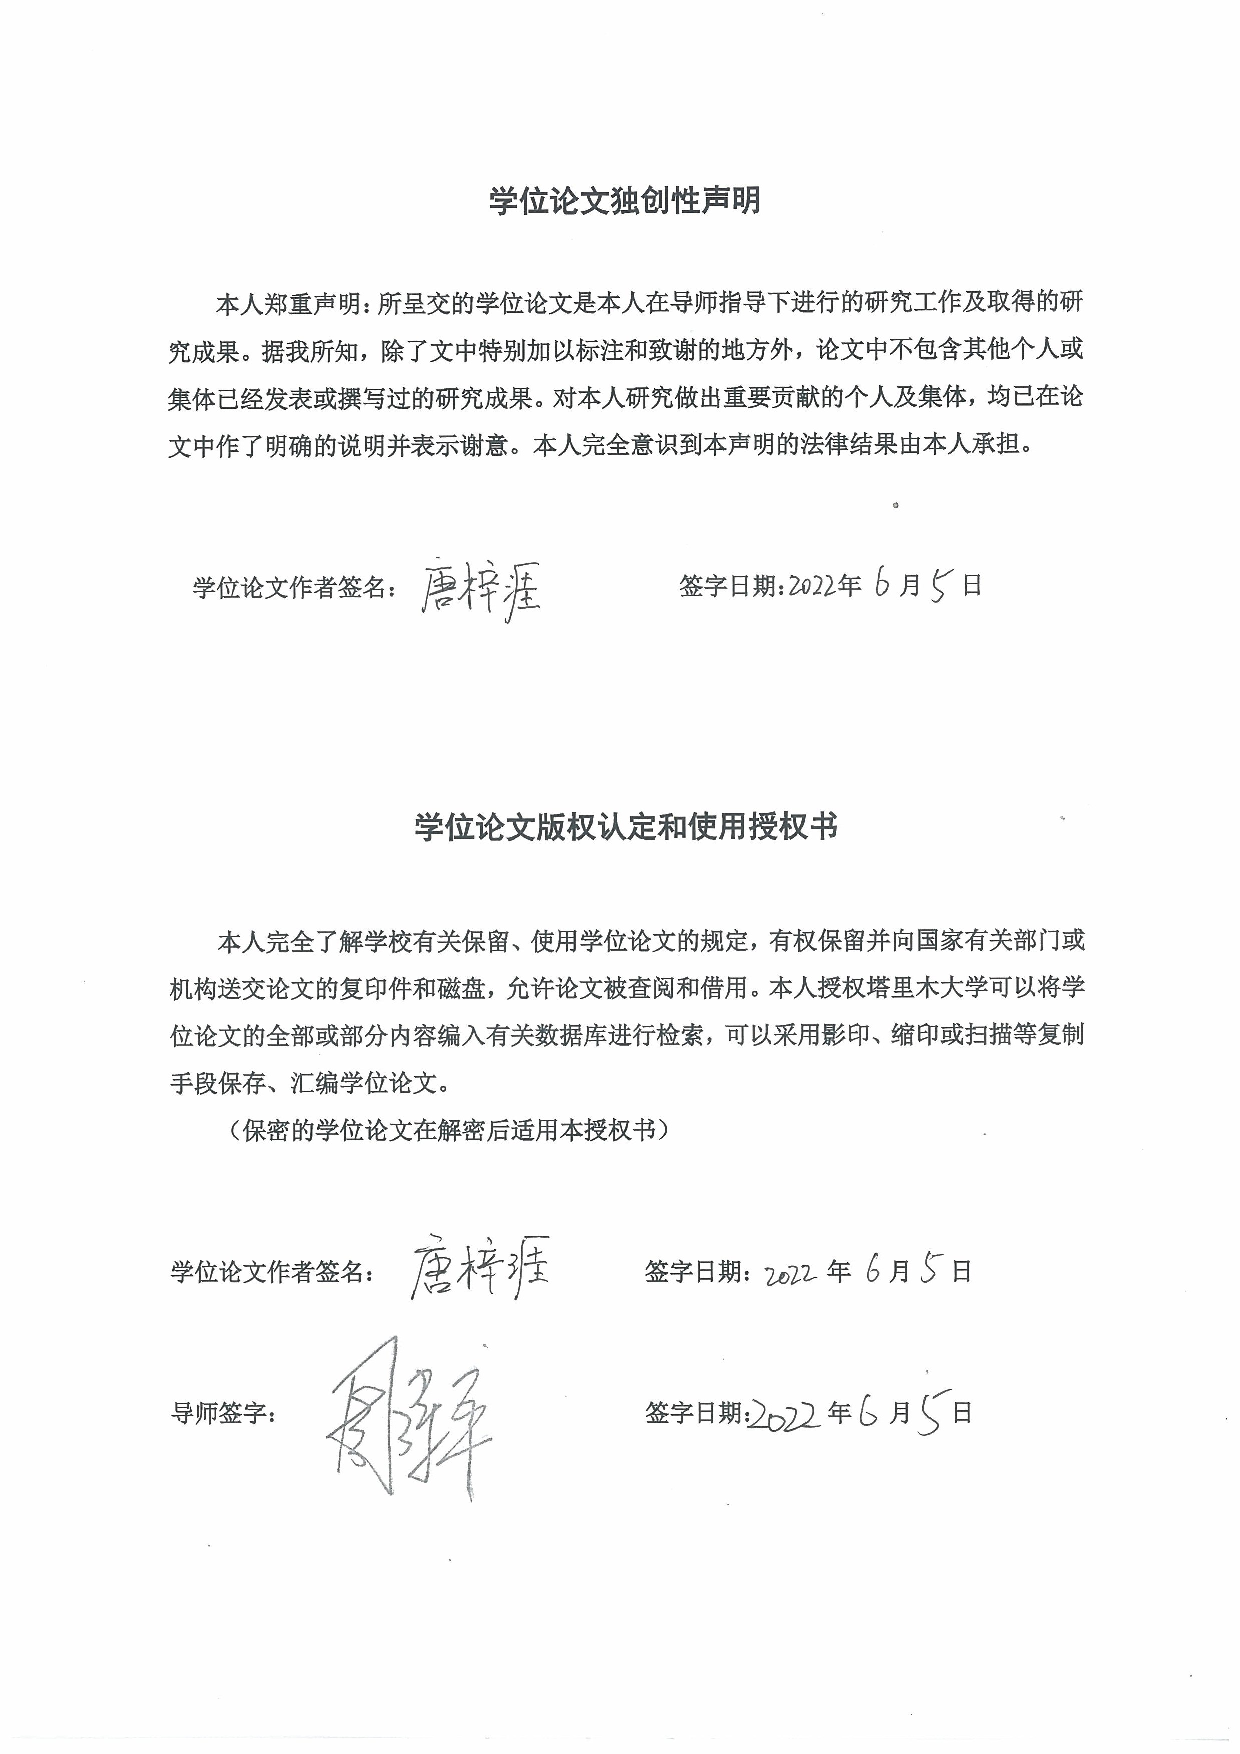
\includepdf{学位论文独创性声明.pdf}
\chapter*{摘要}
无膜栽培技术是解决南疆地区棉田残膜污染的有效手段。
项目拟通过模型模拟定量评价种植密度和灌溉制度对无膜棉生长和产量的影响,
以 Cotton2K 模型为基础,重点解决棉花生长模拟过程中的两个关键科学问题:
\begin{enumerate*}
    \item 棉花不同发育阶段有效光合叶面积指数在冠层的空间分布不一致。
    \item 光能截获、盐分和根系分布对水分运移的耦合影响和定量描述。
\end{enumerate*}
首先,综合考虑热效应和光周期效应模拟物候学发育时间;
其次,建立有效面积指数在冠层空间分布比例与生理发育时间的分段函数方程,改进光能截获模拟精度,构建基于过程的棉花光合生产与干物质积累模型;
再次, IRE 方法改进水分运移方程上下边界条件,采用根系吸水与根长密度分布统一求解的方法,分层计算盐分和根系分布对水分运移的影响,建立考虑冠层光能截获、根系和盐分空间分布的水分运移模型;
最后,量化棉花各器官干物质分配、蕾铃发育与脱落过程,构建棉花干物质分配与产量形成的模拟模型。
% 目录首页不需要页码,但默认目录首页是plain的,所以用empty覆盖
\fancypagestyle{plain}{
  \pagestyle{empty}
}
\tableofcontents
\newpage
\mainmatter
% 章节首页也需要页眉,但默认章节首页是plain的,所以用fancy覆盖
\fancypagestyle{plain}{
  \pagestyle{fancy}
}
\pagestyle{fancy}
\setcounter{page}{1}
%答辩意见
%王德胜
%1. 摘要首句要修改措辞
%2. 参考文献从2号开始,摘要不能有参考文献
%李旭
%1. 结论太少
%张晓
%1. 图片格式
%孟洪兵
%1. 需要在文中体现盐渍化
%2. 露点温度的获取
\begin{spacing}{\fpeval{25 / (12 * 1.2)}}
  \chapter{绪论}\label{chap:intro}
\section{研究背景及意义}
新疆南部地区 (南疆) 日照时间长、光热资源丰富,为优质棉花的生长提供了绝佳的自然条件.
2021 年新疆棉花播种面积 2506.1 千公顷 (全国 3028.1 千公顷),产量 500.2 万吨 (全国 512.9 万吨) \cite{国家统计局关于2021年棉花产量的公告},是我国和世界最具发展前景的优质棉生产基地。
新疆从 1980 年代开始大范围推广使用地膜覆盖技术种植棉花,这一举措被誉为“白色革命”,大幅提高了棉花的生产效率,带来了丰厚的经济效益。%
但残留地膜回收率低,在土壤中难以降解,土壤中残膜量逐年增加,不仅对土壤结构造成破坏,而且对混入残膜的纤维品质也降低了,“白色革命”终成“白色污染”。
中国工程院院士喻树迅团队连续 7 年在南疆多地的试验示范站实现了棉花的无膜化种植,成功培育出了早熟品种“中棉 619”,%
可实现平均亩产 365 公斤\cite{yu2019}。
然而,无膜棉的种植与推广还有诸多问题需要解决,如播种密度和肥水调控等问题急需深入研究。
因此,在南疆干旱区开展无膜棉生长和水分运移模拟研究,%
对指导无膜棉播种日期、播种量、精准灌溉和提高产量具有重要意义。
有效光合叶面积指数发芽后集中在冠层的底部,成熟期集中在顶部,而花期属于均匀分布,%
本文将借鉴成熟的棉花生长模型理论,集中解决有效光合叶面积指数不同发育阶段在棉花冠层分布不一致的问题,提高光能截获和光合作用模拟精度。

\section{国内外研究现状}
\subsection{主要的棉花生长模型}
棉花 (\textit{Gossypium hirsutum L.} 与 \textit{Gossypium barbadense L.})是全球重要的商品作物,为不同行业提供纤维、饲料、食物和潜在的燃料来源。%
棉花纤维被用于从纺织品到纸张、咖啡过滤器和渔网等产品。%
棉籽粉和棉籽壳主要用于反刍牲畜饲料。棉籽油目前被提炼成植物油供人食用,并有可能成为生物燃料。%
我国棉花生产的一个主要问题是生产成本高,需要改进棉花生产方式,以保持棉花在经济上对其他商品作物和替代纤维来源的竞争力。%
为了使棉花生产具有可持续性,还必须考虑水和能源资源的限制。%
通过更明智的灌溉和氮肥管理,更好地了解气候对棉花产量的影响,进一步推进棉花育种和遗传学,更多地采用精准农业技术,以及增加对棉花遗传学与环境管理(GEM)相互作用的了解,可以实现这些改进棉花生产的目标。

作物生长模型以经验公式的形式将作物的生长发育、光合生产、器官建成和产量形成等过程描述出来,%
与环境与栽培管理有机结合,通过计算机程序对作物生长指标动态地进行定量描述。
棉花生产中种植系统模拟模型的开发和应用有着悠久而丰富的历史,从20世纪60年代在美国东南部开始,现已扩展到全球主要的棉花生产地区。%
目前主流的专用棉花生长模型主要有 GOSSYM\cite{baker1976},COTCO2\cite{wall1994},OZCOT\cite{hearn1994},CROPGRO-Cotton\cite{jones2003} 和 Cotton2K\cite{cotton2kv4} 等,%
另外,一些通用的作物生长模型也被用于模拟棉花生长,如 EPIC\cite{williams1989},WOFOST\cite{vanDiepen1989WOFOST},SUCROS\cite{vanittersum2003},GRAMI\cite{ko2005},CropSyst\cite{sommer2008}和 AquaCrop\cite{steduto2009}。
模型的应用领域包括作物用水和灌溉水管理、氮素动力学和肥料管理、遗传学和作物改良、气候学、全球气候变化、精准农业、模型与传感器数据整合、经济学和课堂教学。%
总的来说,在上个世纪重视棉花模型的开发,本世纪以来则越来越重视棉花模型的应用\cite{thorp2014}。%
尽管的最早棉花模型已经有 50 年的历史,但棉花模型之间的对比较少\cite{thorp2014}。%
越来越多的棉花模拟模型被非传统的作物建模者应用,他们不是训练有素的农学家,但希望使用模型进行广泛的经济或生命周期分析。%
尽管这一趋势表明人们对模型的兴趣越来越大,而且模型在各种应用中都有潜在的效用,但这就需要为特定的应用开发具有适当复杂性和易用性的模型,而且需要改进文件和教材来教育潜在的模型用户。%
空间尺度问题也越来越突出,因为最初为田间使用而开发的模型正被用于大面积的区域模拟。%
研究朝着模型与变速控制系统集成的高级目标稳步推进,该系统利用实时作物状态和环境信息,在空间和时间上优化作物投入的应用,同时也考虑潜在的环境影响、资源限制和气候预测。%
总的来说,审查表明在棉花模拟模型开发方面的努力停滞不前,但现有模型在各种研究领域的应用仍然强劲,并继续增长。%


\begin{table}
    \caption{现有棉花生长模拟模型基本信息}\label{tab:overview}
    \small
    \centering
    \begin{tabular}{cp{0.14\linewidth}cccp{0.22\linewidth}}
        \toprule
        名称               & 父代模型         & 编程语言 & 时间步长 & 核心引用                    & 支持决策工具           \\
        \midrule
        GOSSYM             & SIMCOTI SIMCOTII & Fortran  & 日       & \authoryearcite{baker1976}  & COMAX\cite{lemmon1986} \\
        Cotton2K           & GOSSYM CALGOS    & C++      & 小时     & \authoryearcite{cotton2kv4} & 无                     \\
        COTCO2             & KUTUN ALFALFA    & Fortran  & 小时     & \authoryearcite{wall1994}   & 无                     \\
        OZCOT              & SIRATAC          & C\#      & 日       & \authoryearcite{hearn1994}  & APSIM 生态\cite{APSIM} \\
        CSM-CROPGRO-Cotton & CROPGRO-Soybean  & Fortran  & 日       & \authoryearcite{jones2003}  & DSSAT                  \\
        \bottomrule
    \end{tabular}
\end{table}

这些模型通过模拟计算大气、土壤和植物之间的交互作用和水分、能量平衡来实现对棉花生长过程的模拟。%
然而,不同的作物生长模型在选择模拟这些过程的方法和实现细节存在一定差异 (表 \ref{tab:growdev})\cite{thorp2014},%
但主要过程都包括了物候学、光能截获、碳 (C) 同化、呼吸作用、器官形成、生物量积累与分配和胁迫影响等。

一些新发展的通用模型理论和方法也对棉花生长模拟的研究具有重要的推动作用。
由联合国粮食及农业组织 (FAO) 支持的 AquaCrop 模型是模拟水资源管理产量响应的新型通用作物模型\cite{tan2018}。
它基于植物生理学和土壤水分平衡的模拟,取代了粮农组织以前的方法,用于估算与供水有关的作物生产力。
另外,发展和参数化的 WALL 模型也通过聚焦水分在叶片运移用于仿真单叶的水分蒸发\cite{pachepsky2009}。
2021 年最新版本的 SWAP 4.0 版本\cite{swap2021}综合考虑了水、热、冷和盐分胁迫对蒸发蒸腾的影响,%
多尺度 SWAP 模型是否可以改进已提出的棉花模型的水分运移模拟值得深入分析和探讨。

中国作为世界上的主要棉花生产国,对棉花生长模拟的研究发展飞速,%
比较有代表性的是潘学标等开发的 COTGROW\cite{pan1996} 模型,%
此外,南京农业大学的曹卫星教授带领的科研团队\cite{zhang2003,ma2004,chen2006}也分别建立了棉花生育周期和品质形成模拟模型,%
这些模型相比国外的棉花生长模型,加入了如化控、覆膜等我国特有的管理措施。%
然而,由于生长模型的复杂性,对于不同的场景,不同模型之间的表现存在一定的差异性。

\begin{table}
    \small
    \caption{现有棉花生长模拟模型生长和发育阶段模拟}
    \label{tab:growdev}
    \begin{tabular}{p{0.14\linewidth}p{0.14\linewidth}p{0.14\linewidth}p{0.14\linewidth}p{0.14\linewidth}p{0.14\linewidth}}
        \toprule
                   & GOSSYM                                                                       & Cotton2K                                                                     & COTCO2                                                                   & OZCOT                                                                      & CROPGRO-Cotton                                                                                   \\
        \midrule
        物候学     & 根据积温发育叶枝果枝和坐果节,计算果枝、蕾、铃、开铃、坐果节和脱落果实的数量 & 根据积温发育叶枝果枝和坐果节,计算果枝、蕾、铃、开铃、坐果节和脱落果实的数量 & 根据积温发育分生组织、叶原基、叶柄,生长和成熟叶、节间茎段、蕾、铃和开铃 & 根据积温计算坐果节的数量,根据作物承载能力计算蕾、铃、开铃和脱落果实的数量 & 根据光热时间计算出苗、第一片叶、第一朵花、第一个种子、第一次开铃和 90\% 开铃、铃数和脱落果实数量 \\
        植株映射   & 有                                                                           & 有                                                                           & 有                                                                       & 无                                                                         & 无                                                                                               \\
        潜在碳同化 & 冠层尺度辐射截获                                                             & 冠层尺度辐射截获                                                             & 器官尺度生物化学驱动\cite{farquhar1980}                                  & 冠层尺度辐射截获                                                           & 叶片尺度生物化学驱动\cite{farquhar1980}                                                          \\
        呼吸作用   & 使用生物量和温度的经验函数计算                                               & 计算生长和维持呼吸,以及光合呼吸                                             & 计算器官尺度的生长、维持和光合呼吸                                       & 使用基于坐果节数和气温的经验函数                                           & 计算生长和维持呼吸                                                                               \\
        同化分配   & 分配碳同化产物到每个生长器官                                                 & 分配碳同化产物到每个生长器官                                                 & 分配碳同化产物到每个生长器官                                             & 将碳同化产物分配到用于棉铃发育的储存池                                     & 将碳同化产物分配到用于叶、茎、根和铃发育的单一存储池                                             \\
        冠层尺寸   & 计算高度                                                                     & 计算高度                                                                     & 计算茎节长度                                                             & 无                                                                         & 计算高度和宽度                                                                                   \\
        产量要素   & 根据棉铃的质量和尺寸计算纤维质量                                             & 计算纤维质量和种子棉质量                                                     & 计算棉铃质量                                                             & 根据棉铃的质量和尺寸计算纤维质量                                           & 计算棉铃质量、种子棉质量、种子数量和单位种子重量                                                 \\
        胁迫       & 计算水、氮和气温胁迫                                                         & 计算水、氮和气温胁迫                                                         & 计算水和气温胁迫                                                         & 计算水、氮和气温胁迫                                                       & 计算水、氮和气温胁迫                                                                             \\
        \bottomrule
    \end{tabular}
\end{table}

\begin{table}
    \small
    \caption{现有棉花生长模拟模型大气和土壤模拟}\label{tab:atmosoil}
    \begin{tabular}{p{0.14\linewidth}p{0.14\linewidth}p{0.14\linewidth}p{0.14\linewidth}p{0.14\linewidth}p{0.14\linewidth}}
        \toprule
                               & GOSSYM                           & Cotton2K                         & COTCO2                         & OZCOT                        & CROPGRO-Cotton                          \\
        \midrule
        $CO_2$对光合作用的影响 & 有                               & 有                               & 有                             & 无                           & 有                                      \\
        $CO_2$对呼吸作用的影响 & 无                               & 无                               & 有                             & 无                           & 有                                      \\
        蒸腾作用               & \authornumcite{ritchie1972}      & CIMIS 中的改进的 Penman 公式     & 叶片尺度能量平衡与气孔导度耦合 & \authornumcite{ritchie1972}  & \authornumcite{priestley1972,fao56}     \\
        土壤水分               & 2D RHIZOS 模型\cite{lambert1976} & 2D RHIZOS 模型\cite{lambert1976} & 2D 模型                        & \authornumcite{ritchie1972}  & \authornumcite{ritchie1998,ritchie2009} \\
        土壤氮                 & 土壤和植物氮平衡的动态仿真       & 土壤和植物氮平衡的动态仿真       & 无                             & 统计和经验方法预测潜在氮吸收 & \authornumcite{godwin1998,gijsman2002}  \\
        土壤磷                 & 无                               & 无                               & 无                             & 无                           & 有                                      \\
        土壤盐分               & 无                               & 有                               & 无                             & 无                           & 无                                      \\
        渍灾                   & 无                               & 无                               & 无                             & 有                           & 有                                      \\
        涝灾                   & 无                               & 无                               & 无                             & 无                           & 有                                      \\
        \bottomrule
    \end{tabular}
\end{table}
\begin{table}
    \caption{现有的棉花模拟模型和其他应用所模拟的管理实践}\label{tab:agromanagement}
    \begin{tabular}{p{0.14\linewidth}p{0.14\linewidth}p{0.14\linewidth}p{0.14\linewidth}p{0.14\linewidth}p{0.14\linewidth}}
        \toprule
                     & GOSSYM & Cotton2K & COTCO2 & OZCOT & CROPGRO-Cotton \\
        \midrule
        播种日期     & X      & X        & X      & X     & X              \\
        栽培品种选择 & X      & X        & X      & X     & X              \\
        行间距       & X      & X        & X      & X     & X              \\
        间隔行       & X      & X        &        & X     &                \\
        种植密度     & X      & X        & X      & X     & X              \\
        灌溉         & X      & X        & X      & X     & X              \\
        施肥         & X      & X        &        & X     & X              \\
        农作物残留物 &        &          &        &       & X              \\
        耕作         &        & X        &        &       & X              \\
        生长调节剂   & X      & X        &        &       &                \\
        落叶剂       & X      & X        &        &       &                \\
        虫害         & X      & X        & X      & X     & X              \\
        病害         &        & X        &        &       & X              \\
        气候变化     & X      &          & X      &       & X              \\
        耕作顺序     &        &          &        & X     & X              \\
        地理空间分析 &        & X        &        & X     & X              \\
        \bottomrule
    \end{tabular}
\end{table}
\subsection{棉花生长模型的应用研究}

棉花生长模型最基本的目的是预测产量,近几年,国外已经再水分利用效率评价和灌溉管理\cite{baumhardt2014,booker2014,booker2015,modala2015,thorp2015,anapalli2016,attia2016,linker2016,tsakmakis2018,thorp2019,thorp2020,thorp2020a}、
氮磷动态和施肥管理\cite{shumway2012,amin2017,arshad2017,zurweller2019}、%
气象变化响应\cite{abbas2020}、%
品质模拟\cite{ma2005}、%
打顶和生产管理\cite{yang2008}等方面开展了大量研究。
为了不同的研究目的,所选择的模型也存在较大的差异。
国内学者也在产量预测、模型性能评价、水分使用效率评价、品质成分含量模拟、株高生长模拟、水氮耦合效应评价、水盐运移、根系生长模拟和模型敏感性与不确定性分析等方面开展了研究和探索。
然而,在不同生长发育时期,冠层截获的光能在不同空间的分布比例存在一定的差异性和规律性,定量化描述这个过程有望提高光合作用模拟精度。

值得注意的是, GOSSYM 及其后继版本如 Cotton2K 是世界上最成功的棉花模型之一。
Cotton2K 模型基于 GOSSYM 模型的过程公式,借鉴了其他棉花生长模型的算法思想,以小时为单位的高时间分辨率计算水分、物质和能量平衡,%
提高了对干旱地区依赖灌溉的棉花生长模拟的精度和适用性。
虽然模型也考虑了盐分和水分在土壤的分布,然而,使用的 Richards 方程 \cite{richards1931} 计算水分运移过程存在上下边界粗糙的问题 \cite{thorp2014},
而且对于滴灌模式,沿滴灌带垂直方向的根系分布也应被精细的考虑;
另外,实际蒸腾计算过程中对冠层光截获因子的精细模拟也有改进的空间。

\subsection{Cotton2K 模型的应用研究}
Cotton2K 模型是由 Avishalom Marani 教授在美国做访问学者时开发的。
该模型的源代码是用 C++ 编写的,可以免费下载 \cite{cotton2kv4}。
Cotton2K 主要基于 GOSSYM \cite{baker1976,baker1983} 开发,同时也参考了其他棉花生长模型,包括SIMCOTI \cite{baker1972}、SIMCOTII \cite{jones1974}, 和 CALGOS \cite{marani1992a,marani1992b,marani1992c}。
开发 Cotton2K 的主要目的是为如美国西部和以色列这样的干旱、灌溉环境下的棉花生产提供一个更有用的模型。

\authoryearcite{cotton2kv4} 对Cotton2K的历史、主要特征、科学原理和投入要求作了总体描述。
Cotton2K 和 GOSSYM 的根本区别在于对天气数据的要求。
GOSSYM 使用每天的天气数据,而Cotton2K使用每小时的空气温度和湿度、风速和短波的测量值。
而 Cotton2K 使用的是空气温度和湿度、风速和短波辐照度的每小时测量值,或者使用 \authoryearcite{ephrath1996} 的方法,从每日数据中计算出小时值。
每小时的天气值被用来计算相应的每小时水和能量平衡。
这样可以使模型更贴近干旱条件,提高模型在灌溉条件下更准确计算水量平衡的能力\cite{cotton2kv4}。
这些变化的主要影响是提高了蒸发蒸腾的计算精度,同时也影响了相关变量。
此外,使用每日天气数据的时间步长,而不是较短的时间步长所产生的偏差,在在计算能量或水平衡天气参数的相互作用时尤为重要(例如非线性昼夜风速模式和/或风速与太阳辐照度的相互作用驱动蒸散发)\cite{ephrath1996}。
Cotton2K 的其他修改包括地表下滴灌的程序、N 矿化和硝化过程的更新、使用 Michaelis-Menten 程序计算 N 吸收、植物生长和物候功能的更新,以及提供土壤表面和作物冠层温度的能量平衡方程\cite{cotton2kv4}。
总之,增加每小时的天气输入数据后,可以按每小时的时间步长计算和整合微分方程,以实现以下过程 植物蒸腾、土壤水分蒸发、土壤水 再分配、热通量和氮通量,以及在土壤-植物-大气 (soil-plant-atmosphere) 界面的能量和水的交换。
这些修改大大提高了 Cotton2K 在干旱环境中灌溉的实用性和适用性。

在 Cotton2K 中计算过程主要与土壤、植物和环境之间的能量和水的交换有关。
这些过程是基于质量和能量守恒的原则,系统的输入和输出是平衡的,并作为时间的函数。
Cotton2K 模型是为特定的管理农艺投入,包括灌溉、氮肥、脱叶和应用植物生长调节剂。
植物生长和发育基于“胁迫”理论 \cite{grime1977,craine2005,grime2007},包括与空气温度、水、C和N有关的胁迫。
在此种语境下,胁迫是指由于空气温度不理想以及水和营养物质的短缺而限制潜在产量的条件\cite{grime1977}。
使用热单位的概念,植物生长率与环境温度有关\cite{wang1960,peng1989}。
所有植物器官,包括根、茎、叶片和叶柄,以及果实部位(花蕾,棉铃和籽棉)的潜在生长率,都通过胁迫因素与碳和水的源汇关系 (source-sink) 相关联。
源和汇之间的胁迫因子在数值上从1(无胁迫)到0(严重胁迫)不等。
碳胁迫与净碳同化有关(即总光合作用减去光呼吸、生长呼吸和维持呼吸)。
水胁迫与水的蒸腾和运输有关,是一个关于叶片水势的函数。
氮胁迫是基于氮的供应和需求。
在土壤中,Cotton2K 计算来自尿素水解、有机氮的矿化、铵的硝化、硝酸盐的反硝化和可溶性氮的移动的可用氮率。
并且,该模型还计算植物器官(根、茎、叶和果实部位)中的氮。
如果供应不能满足要求,则计算出氮胁迫因子。
所有的供应和需求函数与温度、水、碳和氮有关的所有供求函数都是动态的,且它们的值随时间变化。

在 Cotton2K 中定义一维土壤-植物-大气系统的边界条件是土壤表面以上2米和以下2米。
土壤表面以上的高度(2米)代表测量输入天气数据的屏幕高度,2米的土壤深度代表土壤剖面的下边界。
所需的输入天气数据包括短波辐照度、空气温度、湿度、风速和雨量。
Cotton2K 使用每小时的天气输入值;但是,如果没有每小时的数据,可利用辐射和风速以及空气温度和湿度的最大和最小值的日值计算小时值\cite{ephrath1996}。
对于每次灌溉事件,指定施用方法(喷灌、沟灌和滴灌)、时间(开始和结束)和施用深度。
用户通过指定每个土壤层的数量和厚度来定义土壤剖面的几何形状。
在模拟开始时(即时间=0),用户为每个土壤层指定一个温度、水、有机物、氮和土壤盐度的值。
此外,土壤层被分组为土层,每个土层都有独特的土壤水力特性。
这些属性定义了土壤含水量与水势和导水率的关系,并在 Richards 方程中用于计算土壤剖面中的水分流动。
用户指定地下水位深度和每个耕作事件的日期和深度。
其他固定的参数输入值是位置(纬度、经度和海拔),模拟期的开始和结束,种植和/或出苗日期,以及田间数据(种植密度和行距,包括间隔行)。
描述单个栽培品种的参数会影响物候、生长和发育,并最终影响棉花纤维产量的计算,正如 \authoryearcite{cotton2kv4} 所建议的和 \authoryearcite{booker2013}所展示。
当前版本的 Cotton2K 已经对 Acala SJ-2, GC-510, Maxxa, Deltapine 61, Deltapine 77, Sivon, 新陆早 8 号和中棉 619\cite{zhu2021} 八个棉花栽培品种进行了测试。

Cotton2K模型可以在管理模式下用于灌溉、氮、脱叶和应用生长调节剂。
在这些选项下,Cotton2K 使用预测的天气情景来执行。
用户可以选择几个选项,例如,开始和结束灌溉的日期,施用氮肥的日期,喷洒落叶剂日期,和喷洒植物生长调节剂 (Pix) 的应用。
Cotton2K 的输出被记录在文本文件、图表和土壤图 (soil map)。
文本文件是所有输入和输出值的总结,详细的每日输出和植物图 (plant map)。
图表显示了关键输出变量的动态变化。
而土壤图是二维的的土壤水和氮含量、温度和其他变量的水平和垂直模拟值的图,每个变量都是关于时间的函数。

Cotton2K模型已经被许多研究人员直接和间接地使用和测试。
\authoryearcite{clouse2006} 使用模拟退火法优化了 Cotton2K 的参数,在空间上标定了 Cotton2K 在西德克萨斯州的试验点的土壤参数。
校准后的模型被用来比较特定地点和统一灌溉管理策略。
特定地点灌溉管理的模拟棉纤维产量更高,但产量增加并没有使特定地点灌溉更有利可图。
\authoryearcite{haim2008} 使用Cotton2K模型对以色列的灌溉棉花进行了研究。报告说,在两种气候变化情况下,通过提前两周种植和增加灌溉,可以抵消气候变暖的负面影响。
\authoryearcite{yang2008} 使用了Cotton2K模型,在田间条件下测试了剪枝和打顶的效果,
\authoryearcite{yang2010} 和 \authoryearcite{nair2013} 在有限的水资源条件下优化灌溉分配。
在有限的水资源条件下优化灌溉分配。
\authoryearcite{yang2010} 使用Cotton2K 模型估计华北平原棉花的灌溉用水需求,使用20 年的农艺、水文和气候数据,估算华北平原棉花灌溉需水量。
平均而言,灌溉的棉花生产占该地区总需水量的8\%。
\authoryearcite{nair2011} 使用 Cotton2K 和一个经济模型生成的棉花纤维产量模拟,确定在不同次优灌溉水供应水平下,在棉花不同生长阶段分配灌溉水的经济最优策略。
Cotton2K 还被用来评估将中心枢纽灌溉的棉田划分为灌溉和雨养部分的盈利能力\cite{nair2013}。
这项研究表明,田间分割增加了赤字灌溉棉花的纤维产量和收益。
Cotton2K 模型与计量经济学模型一起使用,评估了棉花生产者对风险的态度对德克萨斯州 高原地区中心枢纽灌溉棉花的最佳灌溉水分配决策的影响 \cite{nair2011}。
结果表明,最佳灌溉水量分配既有增加利润的作用,也有降低风险的作用。
\authoryearcite{nair2013} 模拟德克萨斯高原的德克萨斯州普莱恩维尤市 110 年 68 种不同的灌溉处理的棉花纤维产量,对 Cotton2K 在德克萨斯州高地的应用进行了评估,以分析将中心支流灌溉的棉田划分为灌溉田和旱田的和盈利的影响。
通过对田间进行部分灌溉使得棉花纤维产量和盈利能力得到提高。当可用的灌溉水少和降雨量低的年份,经济效益更高。
\authoryearcite{wang2013} 开发了一个理论框架,用于确定缺水灌溉下棉花的经济最优灌溉水分配,并将该经济模型与 Cotton2K 生成的纤维产量数据一起使用,分析了旨在提高高效灌溉系统采用率的成本分摊计划的节水潜力。
他们得出结论,该计划没有为生产者提供任何节水的激励。
\authoryearcite{booker2013} 将 Cotton2K 纳入一个景观规模的模型中并将其应用于德克萨斯高原主要土壤类型的棉花生产中。
鉴于 Cotton2K 与 GOSSYM 和 CALGOS 模型的相似性,间接地, Cotton2K 中的一些算法已被评估用于广泛的土壤类型。
\authoryearcite{staggenborg1996} 对广泛的土壤和环境条件进行了评估。
\authoryearcite{clouse2006}, \authoryearcite{baumhardt2009} 等人对 Cotton2K 中的一些算法进行了评估。
\authoryearcite{baumhardt2014} 研究了在厄尔尼诺-南方振荡影响下的棉花纤维产量对灌溉管理的响应。
\authoryearcite{thorp2019} 开发了一套全新的方法用于比较模型中蒸发蒸腾算法的效果与性能,从 DSSAT 模型中借鉴 3 种算法,修改 Cotton2K 以替换原始的蒸发蒸腾算法。

上述的研究中基本都是应用 Cotton2K 模型进行分析,极少涉及对模型运行机制的讨论和修改,但最近新的层出不穷的作物生长模型越来越精细,%
Cotton2K 在这个方面亟待改进。

\subsection{发展动态和问题分析}
棉花生长模型的主要发展趋势是从局部到整体,由简单到复杂,由经验性到机理性,由智能化到数字化。%
另外,增强目标性和适用性,构建专门针对某一生产实际问题的专用模型更具有应用价值\cite{thorp2014}。

综上所述,为了服务中棉 619 在南疆地区的无膜栽培推广应用,本文以 Cotton2K 模型为基础,%
重点研究考虑冠层光合作用有效叶面积指数的垂直分布比例的光能截获模拟,以及考虑冠层光能截获、根系和盐分空间分布影响的水分运移模拟,%
建立适合南疆干旱、盐渍化土壤特点的棉花生长模型,
为无膜棉的播种日期、播种量的确定和灌溉制度提供定量化的分析手段。

\section{研究内容和技术路线}

\subsection{研究内容}
\begin{enumerate}
    \item 对 Cotton2K 模型进行修改\\%
          参考 WOFOST-GTC 模型,将 Cotton2K 模型的冠层子模块修改为自上而下的层级结构,每层为 5 cm 高,共 20 层,分层对冠层的光合作用和干物质分配等生理过程进行模拟。%
          同时也修正部分原版模型的错误,例如浮点数计算溢出、干重模拟值为负值等。
    \item Cotton2K 模型的校准与验证\\%
          参考相关文献中对 Cotton2K 模型参数敏感性分析结果,利用 2019 年与 2020 年两年的田间实验数据,使用修改后的 Thorp 方法\cite{thorp2019} 分别对原版模型和修改后的模型的参数进行校准。%
          将 2021 年的田间实验数据作为验证集对校准后的 Cotton2K 进行验证,评估 Cotton2K 模型对中棉 619 的模拟精度。
    \item 中棉 619 冠层垂直方向光能截获时空分布规律\\%
          利用 2019 年至 2020 年生育期内采集的冠层光合有效辐射 (PAR) 数据,将棉花冠层分为 20 个等高的子层,研究棉花冠层垂直方向的的光能截获分布规律。
\end{enumerate}

\subsection{技术路线}

研究总技术路线如图 \ref{fig:roadmap} 所示。%
研究以 Cotton2K 模型为理论依据,利用中棉 619 的田间实验数据探究不同生育期光合有效辐射在冠层垂直方向分布的规律。%
\begin{figure}
    \centering
    \begin{tikzpicture}[
            node distance=1cm,
            every node/.style={fill=white, font=\sffamily},
            align=center
        ]
        % Specification of nodes (position, etc.)
        \node (start) [terminalStart] {开始};
        \node (firstSampling) [data, below left=of start, xshift=-3cm] {对 70 个 Cotton2K \\参数进行 Sobol 取样};
        \node (fieldData) [data, below=of start, yshift=-1.5cm] {田间数据};
        \node (firstSimulation) [process, below=of firstSampling, yshift=-1.5cm] {Cotton2K 模拟};
        \node (firstDatabase) [data, below=of firstSimulation] {12 个输出变量的\\评价指标数据库};
        \node (sa) [process, below=of firstDatabase] {使用 SALib 进行\\Sobol 全局敏感性分析};
        \node (influential) [decision, below=of sa] {S1 > 0.05};
        \node (fixParam) [process, below=of start, right=of influential] {固定参数为默认值};
        \node (secondSampling) [data, below right=of start, xshift=3cm] {对 35 个 Cotton2K \\参数进行多目标优化};
        \node (secondSimulation) [process, below=of secondSampling, yshift=-1.5cm] {Cotton2K 模拟};
        \node (secondDatabase) [data, below=of secondSimulation] {12 个输出变量的\\评价指标数据库};
        \node (moo) [process, below=of secondDatabase] {求解 Pareto 解集};
        \node (prune) [process, below=of moo] {对 Pareto 解集进行剪枝};
        \node (compare) [process, below=of prune] {对不同修改进行统计分析};
        \node (stop) [terminalStop, below=of start, left=of compare] {结束};

        \draw [-latex] (start) -| (firstSampling);
        \draw [-latex] (firstSampling) -- (firstSimulation);
        \draw [-latex] (firstSimulation) -- (firstDatabase);
        \draw [-latex] (firstDatabase) -- (sa);
        \draw [-latex] (sa) -- (influential);
        \draw [-latex] (influential.east) -- (fixParam) node[pos=0.5, inner sep=0]{否};
        \draw [-latex] (influential.west) -- +(-1.5cm,0) node[pos=0.5, inner sep=0]{是} -- +(-1.5cm, 13cm) -| (secondSampling);
        \draw [-latex] (secondSampling) -- (secondSimulation);
        \draw [-latex] (secondSimulation) -- (secondDatabase);
        \draw [-latex] (secondDatabase) -- (moo);
        \draw [-latex] (moo) -- (prune);
        \draw [-latex] (prune) -- (compare);
        \draw (fieldData) -| (firstSimulation);
        \draw (fieldData) -| (secondSimulation);
        \draw [-latex] (fixParam) |- (secondSimulation);
        \draw [-latex] (compare) -- (stop);
    \end{tikzpicture}
    \caption{技术路线图}\label{fig:roadmap}
\end{figure}

\subsection{论文结构}
本论文共 6 章,各章节内容简介如下:

第 \ref{chap:intro} 章,主要介绍了无膜栽培棉花的研究背景及意义、棉花生长模型的研究进展以及该论文的研究内容、技术路线以及论文结构。

第 2 章,主要从试验观测、模型模拟、敏感性分析和多目标优化角度介绍本研究采用的材料与方法。

第 3 章,主要介绍了对 Cotton2K 模型的改进,修改了模型的输入输出、修正部分计算、优化模拟运行效率、跨操作系统编译以及增加分层的冠层子模块。

第 4 章,主要介绍了修改前后的 Cotton2K 模型的敏感性分析结果。

第 5 章,主要介绍了 Cotton2K 的校准与验证、模型修改前后的对比和棉花生长模拟结果。

第 6 章,总结与展望。总结了实验的内容和实验结果,阐述了实验中的不足以及未来的改进方案。

\section{本章小结}
本章首先介绍了棉花在世界和中国经济发展中的重要地位。%
然后阐述了棉花的地膜栽培技术在给我国农业发展带来的巨大经济效益的同时,也给我国带来了残膜污染的问题。%
为了保护和改善农业生态环境,减少农用薄膜是切实可行的手段。%
2017 年末,中国工程院喻树迅院士率领的科研育种团队成功培育出中棉 619,该品种适用于无膜种植。%
随后详细论述了 Cotton2K 模型的发展历史和主要特色。
最后介绍了本文的研究内容、技术路线以及论文结构。

  \chapter{材料与方法}


% Drawing part, node distance is 1.5 cm and every node
% is prefilled with white background
\begin{tikzpicture}[
        node distance=1cm,
        every node/.style={fill=white, font=\sffamily},
        align=center
    ]
    % Specification of nodes (position, etc.)
    \node (start) [terminalStart] {开始};
    \node (firstSampling) [data, below left=of start, xshift=-3cm] {对 70 个 Cotton2K \\参数进行 Sobol 取样};
    \node (fieldData) [data, below=of start, yshift=-1.5cm] {田间数据};
    \node (firstSimulation) [process, below=of firstSampling, yshift=-1.5cm] {Cotton2K 模拟};
    \node (firstDatabase) [data, below=of firstSimulation] {12 个输出变量的\\评价指标数据库};
    \node (sa) [process, below=of firstDatabase] {使用 SALib 进行\\Sobol 全局敏感性分析};
    \node (influential) [decision, below=of sa] {S1 > 0.05};
    \node (fixParam) [process, below=of start, yshift=-10cm] {固定参数为默认值};
    \node (secondSampling) [data, below right=of start, xshift=3cm] {对 35 个 Cotton2K \\参数进行 Sobol 取样};
    \node (secondSimulation) [process, below=of secondSampling, yshift=-1.5cm] {Cotton2K 模拟};
    \node (secondDatabase) [data, below=of secondSimulation] {12 个输出变量的\\评价指标数据库};
    \node (moo) [process, below=of secondDatabase] {求解 Pareto 解集};
    \node (prune) [process, below=of moo] {对 Pareto 解集进行剪枝};
    \node (compare) [process, below=of prune] {对不同修改进行统计分析};
    \node (stop) [terminalStop, below=of start, yshift=-11.7cm] {结束};

    \draw [-latex] (start) -| (firstSampling);
    \draw [-latex] (firstSampling) -- (firstSimulation);
    \draw [-latex] (firstSimulation) -- (firstDatabase);
    \draw [-latex] (firstDatabase) -- (sa);
    \draw [-latex] (sa) -- (influential);
    \draw [-latex] (influential.east) -- (fixParam) node[pos=0.5, inner sep=0]{否};
    \draw [-latex] (influential.west) -- +(-1.5cm,0) node[pos=0.5, inner sep=0]{是} -- +(-1.5cm, 13cm) -| (secondSampling);
    \draw [-latex] (secondSampling) -- (secondSimulation);
    \draw [-latex] (secondSimulation) -- (secondDatabase);
    \draw [-latex] (secondDatabase) -- (moo);
    \draw [-latex] (moo) -- (prune);
    \draw [-latex] (prune) -- (compare);
    \draw (fieldData) -| (firstSimulation);
    \draw (fieldData) -| (secondSimulation);
    \draw [-latex] (fixParam) |- (secondSimulation);
    \draw [-latex] (compare) -- (stop);
\end{tikzpicture}



\section{实验观测}
试验区位于南疆地区阿拉尔市塔里木大学灌溉试验站 (\ang{81;11;46}E, \ang{40;37;28}N)。
\begin{figure}
    \centering
    \includegraphics[scale=0.4]{research_site.png}
    \caption{试验站所在位置}
\end{figure}
灌溉实验按照田间实验设计,采用滴灌方式,根据 SWAP 模型\cite{swap2021}的精准灌溉工具,通过气象数据,土壤数据和棉花生长数据计算每日的实际蒸发蒸腾量 ($ET_c$),按照水分需求进行灌溉。
设计三个灌溉水平,标准亏损灌溉 75\% $ET_c$,90\% $ET_c$ 和 100\% $ET_c$。
另外,设计一个经验灌溉水平,灌溉定额 $\mathrm{280 m^3 / 667m^2}$,生育期滴水总计 14 次。
项目中不研究其他营养对棉花生长的影响,所以 N、P、K 肥按照经验值随滴灌施入,测土施肥,各小区施肥量统一,$N$-$P_2O_5$-$K_2O$ 按照 250-100-50 $\mathrm{kg/hm^2}$ 的量进行施肥。
播种日期设计 2 个水平,分别为铺设地膜的棉花播种后第 10 和 15 天,根据出苗率补充到设计的种植密度,并记录补苗日期。
第一年设计三个种植密度,理论密度分别为 15000, 16000 和 17000 株/$\mathrm{hm^2}$。
第二年到第三年根据第一年的模拟结果进行适当调整。
共 24 个处理,进行安全区组设计,每个小区 0.25 亩,每个实验三次重复。

\subsection{气象数据}

该模型所需的每日气象数据包括太阳辐射 ($langley$),最高和最低温度 (℃) 和降水 (mm) 以及2米高度的风速 (km/h)。

\begin{table}
    \caption{Cotton2K 模型所需输入每日气象数据}\label{tab:meteorology}
    \small
    \centering
    \begin{tabular}{cccc}
        \toprule
        名称         & 解释                     & 单位                                              & 是否必须 \\
        \midrule
        太阳辐射强度 & 大气下垫面短波辐射强度   & $\mathrm{langley} = 0.04184\ \mathrm{MJ\ m^{-2}}$ & 是       \\
        最高气温     & 2 m 最高气温             & ℃                                                 & 是       \\
        最低气温     & 2 m 最低气温             & ℃                                                 & 是       \\
        露点温度     & 空气冷却达到饱和时的温度 & ℃                                                 & 否       \\
        降水         & 24 小时内降水            & mm                                                & 是       \\
        风速         & 2 m 风速                 & km/h                                              & 否       \\
        \bottomrule
    \end{tabular}
\end{table}

当露点温度不可得时,可通过公式 \ref{eq:dewpoint} 估算而得。

\begin{equation}\label{eq:dewpoint}
    T_{dew} = \begin{cases}
        SitePar_5                                                            & T_{\max} < 20        \\
        \frac{(40 - T_{\max}) * SitePar_5 + (T_{\max} - 20) * SitePar_6}{20} & 20 \le T_{\max} < 40 \\
        SitePar_6                                                            & T_{\max} \ge 40      \\
    \end{cases}
\end{equation}

式中,$T_{dew}$ 为露点温度 (℃),$T_{\max}$ 为最高气温 (℃),$SitePar_5$ 与 $SitePar_6$ 为用户提供输入,与试验站相关。

当每日风速数据不可得时,使用年平均风速代替。

\begin{figure}
    \centering
    \includegraphics[scale=0.5]{climate.png}
    \caption{2019-2021年试验站棉花生长期主要气象数据}
\end{figure}

冠层温湿度由精创 RC-4HA 收集,设置取样间隔为 0.5 小时。

\subsection{光能截获率}

在2019年使用LI-6400XT便携式光合作用系统,在2020年使用 LI-191R 线量子传感器和 LI-1500 光传感器在每10天的晴天中午13点至15点之间收集光截获数据。
行内空间被划分为网格,5个水平列和根据植物高度分为6层,每个网格的宽度相等,高度为 20 厘米,然后用设备测量每个网格的照度。
光截获量的计算方法是:同一水平层中各网格的平均光照度减去比率,参见公式\ref{eq:measured_li}。

\begin{equation}\label{eq:measured_li}
    LI_{i} = 1 - \frac{\sum^5_{j=1} I_{i,j}}{\sum^5_{j=1} I_{i+1,j}} \quad \mathrm{for} i \in {1,2,\dots,6}
\end{equation}

式中, $LI_{i}$ 为第 $i$ 层的光能截获率, $I_{i,j}$ 是第 $i$ 层第 $j$ 列网格的光照强度, $I_{i+1,j}$ 为上层网格的光照强度。

\subsection{土壤含水量与温度}

土壤温度由 Thermochron® iButton®器件(DS1921G) 收集,设置取样间隔为 2 小时。

\subsection{棉花生理指标}
试验记录内容主要包括:
\begin{enumerate}
    \item 生育期:详细记录棉花播种、出苗、现蕾、开花和吐絮期出现时间,均以全田 50\% 棉株达到发育要求为标准;
    \item 株式图:每 10 天记录一次株式图,内容有株高、叶片数、果枝数、果节数、蕾、花、小铃、大铃及吐絮铃个数与部位等;
    \item 叶面积指数和光合有效辐射:每 10 天结合干物质测定,取全株叶片,用扫描法测定冠层垂直方向 20 个深度和水平 8 个网格的叶面积指数。使用 SunScan冠层分析仪(Delta 公司,英国)测定不同垂直和水平方向的光合有效辐射 PAR 和叶面积指数;
    \item 光合作用:每 10 天测试一次,使用 LI6400XT 便携式光合作用测试仪分层测试净光合速率、气孔导度、胞间 CO2 浓度和蒸腾速率以及光响应曲线;
    \item 干物质积累和分配:每 10 天取样一次,每次取样在苗期取 10 株样品,开花期后每次取 5 株,样品在 80℃下烘干至恒重后,分别测定根、茎、叶、蕾、花、小铃和大铃等各器官的干物质重量;
    \item 产量构成因素:测定棉花籽棉产量、衣分、铃重和纤维重量;
    \item 根系:每隔 10 天取样,在 0-100cm 土壤深度和距棉行 0-40cm 内各 5cm间隔分别用根钻取带根土样,冲根器冲洗根后,用扫描仪扫描成 TIF 图像文件,再采用 DT-SCAN 图像分析软件,计算根系长度、密度、直径和表面积等指标;
    \item 土壤水分:每周取样测定一次土壤容积含水量(20 $\times$ 8 网格),另外,使用矫正后的土壤水分和温度自动记录仪 (HOBO H21-002, United States) 分 10 层实时监测 0-100cm 深度的土壤水分含量;
    \item 土壤盐分(电导率):每周取样在实验室处理后采用 DDS-307 电导率仪测量,折算成土壤盐分含量;
    \item 其他土壤参数:土壤田间持水率、容积密度、枯萎点含水率、饱和土壤含水率、土壤水响应曲线和渗透系数等可直接取样带回实验室进行测量,同步记录灌溉日期和灌溉量;
    \item 土壤蒸发与棉花蒸腾:采用小型蒸渗仪测量蒸发,棉花蒸腾通过水量平衡原理计算;
    \item 气象数据:由塔里木灌溉试验站气象数据提供,包括 15 分钟间隔的温度、湿度、辐射、风速、降雨和气压数据等。
\end{enumerate}

所获数据用 Python 进行统计分析,利用 Duncan 新复极差检验进行差异显著检验 $(p = 0.05)$。

\subsection{棉花水分利用效率}
水分利用效率 (Water use efficiency, WUE) 是节水农业重要指标,高水平的 WUE 是干旱区农业持续发展的关键所在。
WUE 包括灌溉水利用效率,降水利用效率和作物水分利用效率。
由于研究区降水稀少,本文仅分析灌溉水利用效率和作物水分利用效率。

棉花水分利用效率 ($WUE_{ET}$) 和灌溉水分利用效率 ($IWUE$) 计算公式如下:

\begin{equation}
    WUE_{ET} = Y / ET_c
\end{equation}

\begin{equation}
    IWUE = (Y - Y_n) / I
\end{equation}

式中 $Y$ 为皮棉产量 ($\mathrm{kg\ ha^{-1}}$),
$Y_n$ 为无灌水条件下棉花皮棉产量 ($\mathrm{kg\ ha^{-1}}$),
$ET_c$ 为生育期棉花蒸散量,
$I$ 为灌水量 (mm)。
\subsection{棉花蒸散量计算}

各处理耗水量采用水量平衡公式计算:

\begin{equation}
    ET_c = R + I - F + Q - S + \Delta W
\end{equation}

式中 $ET_c$ 为作物蒸发蒸腾量 (mm),
$R$ 为降水量 (mm),
$I$ 为灌水量 (mm),
$F$ 为地表径流量 (mm),考虑到地下埋管滴灌棉田实验期间无地表径流发生,此处取 $F = 0$
$Q$ 为地下水补给量 (mm),实验资料表明 110 \~ 130 cm 深处土壤水分变化不明显,因此做简化处理,取 $Q = 0$,
$\Delta W$ 为土壤储水变化量 (mm),
$S$ 为深层渗漏量(mm),实验田灌水量通过水量平衡方程计算确定,不存在深层渗漏,故 $S=0$;
$\Delta W$ 为土壤贮水量的减少量(mm):

\begin{equation}
    \Delta W = W_i - W_{i+1}
\end{equation}

式中:$W_i$ 和 $W_{i+1}$ 分别为第 $i$ 个时段初和时段末计划湿润层内的土壤贮水量 (mm)。
为方便水量平衡计算,将含水率换算为以 mm 为单位的土壤贮水量 $W$ :

\begin{equation}
    W = 10 \cdot \theta \cdot \gamma \cdot h
\end{equation}

式中:$W$ 为土壤贮水量(mm),$\theta$ 为计划湿润层内土壤质量含水率 (\%),$\gamma$ 为土壤体积质量 ($\mathrm{g cm^{-3}}$),$h$ 为计划湿润层深度 (cm)。

\section{模型模拟}
\subsection{模型改进}

分析叶面积指数、叶倾角和方位角的空间分布规律及光能截获分布,冠层深度拟分为 20 层,每层占棉花总高度的 5\%,水平方向根据棉花冠幅考虑 8 个网格,共 160 个冠层空间。
首先,计算每一层的有效叶面积指数,
其次,定量化每一层与最顶部冠层的光合叶面积指数的比例($PAI_{\%,i}$),重新积分计算有效总光合叶面积指数,
最后,重新驱动 Cotton2K 模型,模拟干物质积累,每一层的 $PAI_{\%,i}$ 通过公式 \ref{eq:pai} 计算
\begin{equation}
    \label{eq:pai}
    PAI_{\%,i} = 1 - (1 - x_i^\alpha)^\beta
\end{equation}
$PAI_{\%,i}$ 是第 $i$ 层截获 $PAI$ 与最顶部冠层 $PAI$ 的比值,$x_i$ 是冠层深度的百分比,
研究中分 20 层,所以最顶层等于 0.05,最底层等于 1。$\alpha$ 和 $\beta$ 根据不同生长发育时期实际观测的每层 $PAI$ 和冠层顶部的 $PAI$ 确定,分段拟合。

首先,IRE 方法改进水分运移方程的上下边界条件,与根系吸水模型耦合,研究土体 100cm,厚度分层 5cm,水平方向间距 5cm。
其次,根据根长密度分布函数计算每个土层空间的根长密度,并使用 SWAP 模型推荐的方法计算潜在蒸发蒸腾量,分配到每一个土层空间。最后,以每小时时间步长应用 IRE 方法离散土壤蒸发、根系吸水和水盐运移过程。
具体步骤如下:


潜在作物蒸腾与土壤蒸发的计算如公式\ref{eq:E_p}和公式\ref{eq:T_p}
\begin{equation}
    \label{eq:T_p}
    T_p = \frac{
        (1 - W_{frac}) \{ V_c \frac{\Delta_v}{\lambda_w} (R_n - G) + \frac{p_1 \rho_a C_a}{\lambda_w} (\frac{e_{sat} - e_a}{r_{a,can}}) \}
    }{
        \Delta_v + \gamma_a(1 + \frac{ r_{s,\min} }{ r_{a,can} LAI_{eff} })
    }
\end{equation}
\begin{equation}
    \label{eq:E_p}
    E_p = \frac{
        (1 - V_c) \frac{\Delta_v}{\lambda_w} (R_n - G)
        + \frac{p_1 \rho_a C_a}{\lambda_w} (\frac{e_{sat} - e_a}{r_{a,can}})
    }{
        \Delta_v + \gamma_a (1 + \frac{r_{soil}}{r_{a,soil}})
    }
\end{equation}

\subsection{模型参数化}
本文采用 2019-2020 连续 2 年的棉花实验数据对 Cotton2K 模型进行参数化。
其中作物生长参数如叶面积指数 (LAI),株高,干物质积累和主茎节数通过实验得到。
土壤参数如土壤水分、盐分初始值由实验得到;饱和导水率,Van-Genuchten
公式参数 $(\alpha, \beta)$ 等参数由率定得到;气象参数取自阿拉尔气象站;
作物参数和水分胁迫参数由率定得到。

\section{多目标优化}
NSGA-III 的基本框架类似于原始的 NSGA-II 算法 \cite{NSGA2},其选择运算符有重大变化。
但是,与 NSGA-II 不同的是, NSGA-III 中种群成员间多样性的维持是通过提供和自适应更新一些分布良好的参考点来帮助的。
为了完整起见,首先对原始的 NSGA-II 算法进行简要描述。
考虑 NSGA-II 算法的第 $t$ 代,假设这一代的父代种群为 $P_t$,其规模为 $N$ ,而由 $P_t$ 产生的子代种群为 $Q_t$,有 $N$ 个成员。
第一步是从结合的亲代和子代种群 $R_t = P_t \cup Q_t$(大小为 $2N$ )中选择最好的 $N$ 个成员,从而能够保留亲代种群的精英成员。
为了实现这一目标,首先根据不同的非同源等级($F_1$、$F_2$等)对组合群体 $R_t$ 进行排序。
然后,从 $F_1$ 开始,每次选择一个非同化水平来构建一个新的种群 $S_t$ ,直到St的大小等于 $N$ 或首次超过 $N$。
因此,从第 $(l+1)$ 级开始的所有解决方案都被拒绝在组合群体 $R_t$ 中。
在这种情况下,只有那些能使第l层前面的多样性最大化的解决方案被选择。
在 NSGA-II 中,这是通过一个计算效率高但近似的利基 (niche) 保护算子来实现的,该算子将每个最后一级成员的拥挤距离计算为两个相邻解决方案之间的客观归一化距离之和。
此后,具有较大拥挤距离值的解决方案被选中。
在 NSGA-III 中,用以下方法取代拥挤距离算子。

\subsection{将种群按非支配等级分类}

上述利用通常的支配原则\cite{chankong1983}识别非支配前沿的程序也被用于NSGA-III。
如果 $|St|=N$ ,则不需要进一步的操作,下一代从$P_t+1=S_t$开始。
对于 $|St|>N$,从一到 ($l-1$) 个前沿的成员已经被选中,即 $P_{t+1}= \cup_{i=1}^{l-1} F_i$ ,剩下的 $(K=N-|Pt+1|)$ 人口成员从最后的前沿 $F_l$ 中选择。
在下面几个小节中描述其余的选择过程。

\subsection{确定超平面上的参考点}

如前所述, NSGA-III 使用一组预定义的参考点来确保获得的解决方案的多样性。
所选择的参考点既可以以结构化的方式预定义,也可以由用户优先提供。
在没有任何偏好信息的情况下,可以采用任何预定义的结构化的参考点放置,但实践中常常使用 Das和Dennis的\cite{das&dennis2000}系统方法1,
将点放置在一个归一化的超平面--一个 ($M-1$) 维的单位单纯线上,该平面对所有目标轴的倾斜度相同,在每个轴的截距为1。
如果沿每个目标考虑 $p$ 个划分,那么在一个 $M$ 目标问题中,参考点的总数 ($H$) 由以下公式给出

\begin{equation}\label{eq:H}
    H = \begin{pmatrix}
        M + p - 1 \\
        p
    \end{pmatrix}
\end{equation}

例如,在一个三目标问题 ($M = 3$) 中,参考点被创建在一个三角形上,顶点在 $(1, 0, 0)$,$(0, 1, 0)$,$(0, 0, 1)$。
如果为每个目标轴选择四个分部 $(p=4)$, $H = (\begin{smallmatrix}
        3+4-1\\
        4
    \end{smallmatrix})$ 或 $15$ 个参考点将被创建。
为清楚起见,这些参考点显示在图 \ref{fig:refPoints} 中。
在 NSGA-III 中,除了强调非支配性的解决方案外,还强调在某种意义上与这些参考点中的每一个相关的人口成员。
由于上述创建的参考点广泛分布在整个归一化超平面上,因此获得的解决方案也可能广泛分布在帕累托最优前沿或附近。
在用户提供一组首选参考点的情况下,理想情况下,用户可以在归一化超平面上标记 $H$ 个点,或者为此给出任何 $H$ 个 $M$ 维的向量。
所提出的算法有可能找到与所提供的参考点相对应的接近帕累托最优的解决方案,从而使这种方法可以更多地从决策和多目标优化的综合应用角度来使用。
该程序在算法 \ref{alg:NSGA3} 中提出。
\begin{figure}
    \tdplotsetmaincoords{75}{135}
    \centering
    \begin{tikzpicture}
        [tdplot_main_coords,
            axis/.style={-stealth,thick},
            vector/.style={-stealth,very thick}]
        \draw[axis] (0,0,0) -- (5,0,0) node[anchor=east]{$f1$};
        \draw[axis] (0,0,0) -- (0,5,0) node[anchor=west]{$f2$};
        \draw[axis] (0,0,0) -- (0,0,5) node[anchor=west]{$f3$};
        \filldraw[fill=gray,fill opacity=0.8] (0,0,4)--(4,0,0)--(0,4,0)--cycle;
        \draw[-stealth,very thick] (0,3,3) node[anchor=west]{归一化平面} -- (0.5,1.25,2.25);
        \draw[-stealth,very thick] (2,3,0) node[anchor=west]{理想点} -- (0,0,0);
        \fill(4,0,0) circle (2pt) node[anchor=south] {1};
        \fill(3,1,0) circle (2pt);
        \fill(3,0,1) circle (2pt);
        \fill(2,2,0) circle (2pt);
        \fill(2,1,1) circle (2pt);
        \fill(2,0,2) circle (2pt);
        \fill(1,3,0) circle (2pt);
        \fill(1,2,1) circle (2pt);
        \fill(1,1,2) circle (2pt);
        \fill(1,0,3) circle (2pt);
        \draw[-stealth,very thick] (3,0,4) node[anchor=east]{参考点} -- (1,0,3);
        \fill(0,4,0) circle (2pt) node[anchor=south] {1};
        \fill(0,3,1) circle (2pt);
        \fill(0,2,2) circle (2pt);
        \fill(0,1,3) circle (2pt);
        \fill(0,0,4) circle (2pt) node[anchor=south east] {1};
        \draw[vector] (0,0,0) -- (3,1.5,1.5) node[anchor=south]{参考向量};
    \end{tikzpicture}
    \caption{15个结构化参考点显示在归一化参考平面上,适用于$p=4$的三目标问题}\label{fig:refPoints}
\end{figure}


\begin{algorithm}\label{alg:NSGA3}
    \caption{NSGA-III 第 t 代的过程}
    \KwIn{$H$ 构造的参考点 $Z^s$ 或提供的目标点 $Z^a$, 父代种群 $P_t$}
    \KwOut{$P_{t+1}$}

    $S_t = \emptyset, i = 1$\\
    $Q_t$ = 重组+变异($P_t$)\\
    $R_t = P_t \cup Q_t$\\
    $(F_1, F_2, \dots)$ = 非支配排序($R_t$)\\
    \Repeat{$|S_t \ge N|$}{$S_t = S_t \cup F_i$ 且 $i = i + 1$}
    包含父代的 Pareto 前沿: $F_l = F_i$\\
    \eIf{$|S_t| = N$}{
    $P_{t+1} = S_t$, break
    }{
    $P_{t+1} = \cup^{l-1}_{j=1} F_j$\\
    从 $F_l$ 中选点: $K = N - |P_{t+1}|$\\
    归一化目标并创建参考集 $Z^r$: $\mathtt{Normalize}(\mathbf{f}^n, S_t, Z^r, Z^s, Z^a)$\\
    将 $S_t$ 的每个成员 $\mathbf{s}$ 与参考点相关联: $[\pi(\mathbf{s}), d(\mathbf{s})] =\mathtt{Associate}(S_t, Z^r)$
    \tcc{$\pi(\mathbf{s})$: 最近参考点, $d$: $\mathbf{s}$ 与 $\pi(\mathbf{s})$ 之间的距离}
    计算参考点的利基 (niche) 数 $j \in Z^r$: $\rho_j = \sum_{\mathbf{s}\in S_t/F_l}((\pi(\mathbf{s})) ? 1 : 0 )$\\
    一次从 $F_l$ 选取 $K$ 个成员构建 $P_{t+1}$: $\mathtt{Niching}(K, \rho_j, \pi, d, Z^r, F_l, P_{t+1})$
    }
\end{algorithm}
\subsection{种群成员的适应性归一化}
首先,$S_t$种群的理性点是由在$\cup_{\tau=0}^t S_{\tau}$中的每个目标函数$i =1,2,\dots,M$的最小值 ($z_i^{\min}$) 通过构建理想点%
$\overline{z} = (z_1^{\min}, z_2^{\min},\dots,z_M^{\min})$ 来确定的。%
然后,$S_t$ 的每个目标值通过用$z_i^{\min}$减去目标$f_i$来翻译,这样,翻译后的 $S_t$ 的理想点就成为一个零矢量。%
接着,通过寻找使相应的成就标化函数 (由$f'_i(\mathbf{x}) = f_i(\mathbf{x}) - z_i^{\min}$和接近第$i$个目标轴的权重向量形成) 最小的解 $(x \in S_t)$,%
来确定每个(第$i$个)目标轴中的极端点 ($z^{i,\max}$)。
随后,这些$M$个极端向量被用来构成一个$M$维的超平面。%
接下来可以计算出第$i$个目标轴和线性超平面的截距$a_i$(见图\ref{fig:formingHyperPlane})。%
\begin{figure}
    \tdplotsetmaincoords{45}{120}
    \centering
    \begin{tikzpicture}
        [tdplot_main_coords,
            cube/.style={very thick,black},
            grid/.style={very thin,gray},
            axis/.style={-stealth,thick},
            vector/.style={-stealth,very thick},
            annotation/.style={fill=white,font=\footnotesize,inner sep=1pt}]
        \draw[axis] (0,0,0) -- (6,0,0) node[anchor=east]{$f'_1$};
        \draw[axis] (0,0,0) -- (0,6,0) node[anchor=west]{$f'_2$};
        \draw[axis] (0,0,0) -- (0,0,6) node[anchor=west]{$f'_3$};
        \foreach \coo in {2,4}
            {
                \draw (\coo, 0, 0) node[anchor=east] {\fpeval{\coo/2}} -- (\coo, 0.25, 0);
                \draw (0, \coo, 0) node[anchor=south] {\fpeval{\coo/2}} -- (0.25, \coo, 0);
                \draw (0, 0, \coo) node[anchor=east] {\fpeval{\coo/2}} -- (0, 0.25, \coo);
            }
        \foreach \coo in {1,3,5}
            {
                \draw (\coo, 0, 0) -- (\coo, 0.125, 0);
                \draw (0, \coo, 0) -- (0.125, \coo, 0);
                \draw (0, 0, \coo) -- (0, 0.125, \coo);
            }
        \draw[thick] (0,0,5.2)--(4.4,0,0)--(0,3.5,0)--cycle;
        \draw (4.4,0,0)--(4.4,-1,0);
        \draw (0,0,0)--(0,-1,0);
        \draw (0,0,5.2)--(0,-1,5.2);
        \draw (0,0,0)--(-1,0,0);
        \draw (0,3.5,0)--(-1,3.5,0);
        \draw[arrows=<->] (0,-0.8,0)--(2.2,-0.8,0) node[annotation] {$a_1$}--(4.4,-0.8,0);
        \draw[arrows=<->] (-0.8,0,0)--(-0.8,1.75,0) node[annotation] {$a_2$}--(-0.8,3.5,0);
        \draw[arrows=<->] (0,-0.8,0)--(0,-0.8,2.6) node[annotation] {$a_3$}--(0,-0.8,5.2);
        \fill(\fpeval{4.4*0.1},\fpeval{3.5*0.1},\fpeval{5.2*0.8}) circle (2pt);
        \fill(\fpeval{4.4*0.05},\fpeval{3.5*0.8},\fpeval{5.2*0.15}) circle (2pt);
        \fill(\fpeval{4.4*0.8},\fpeval{3.5*0.1},\fpeval{5.2*0.1}) circle (2pt);
        \draw[dash pattern=on 5pt off 5pt] (\fpeval{4.4*0.1},\fpeval{3.5*0.1},\fpeval{5.2*0.8}) node[anchor=south west] {$z^{3,\max}$}--(\fpeval{4.4*0.05},\fpeval{3.5*0.8},\fpeval{5.2*0.15}) node[anchor=south west] {$z^{2,\max}$}--(\fpeval{4.4*0.8},\fpeval{3.5*0.1},\fpeval{5.2*0.1}) node[anchor=west] {$z^{1,\max}$}--cycle;
    \end{tikzpicture}
    \caption{以三目标问题为例,计算截距,然后从极端点形成超平面的程序}\label{fig:formingHyperPlane}
\end{figure}
要特别注意处理退化的情况和非负的截距。%
再然后,目标函数可以被规范化为
\begin{equation}\label{eq:normalize}
    f_i^n (\mathbf{x})= \frac{f_i'(x)}{a_i},\ \mathrm{for}\ i = 1, 2, \dots, M.
\end{equation}
请注意,现在每个归一化目标轴的截点都在$f_i^n = 1$,用这些截点构建的超平面将使$\sum^M_{i=1} f_i^n = 1$。
在结构化参考点 (其中有$H$个) 的情况下,用Das和Dennis\cite{das&dennis1998}的方法计算的原始参考点已经位于这个归一化的超平面上。%
在用户偏爱参考点的情况下,参考点只需使用 \ref{eq:normalize} 映射到上述构建的标准化超平面上。%
由于归一化程序和超平面的创建是在每一代使用从模拟开始时发现的极端点来完成的,%
因此 NSGA-III 程序在每一代都能自适应地保持 $S_t$ 成员所跨越空间的多样性。%
这使得 NSGA-III 能够解决具有帕累托最优前沿的问题,其目标值可以有不同的比例。%
该程序也在算法 \ref{alg:normalize} 中进行了描述。
\begin{algorithm}
    \caption{$\mathtt{Normalize}(\mathbf{f}^n, S_t, Z^r, Z^s, Z^a)$过程}\label{alg:normalize}
    \KwIn{$S_t$, $Z^s$ (构造点) 或 $Z^a$ (提供点)}
    \KwOut{$\mathbf{f}^n$, $Z^r$ (归一化的超平面上的参考点)}

    \For{$j = 1 \mathbf{to} M$}{
    计算理想点: $z_j^{\min} = \min_{\mathbf{S}\in S_t} f_j(s)$
    翻译目标: $f_j'(\mathbf{s}) = f_j(\mathbf{s}) - z_j^{\min} \quad \forall \mathbf{s} \in S_t$
    计算极点: $(\mathbf{z}^{j,\max}, j = 1, \dots, M)$ of $S_t$
    }

    计算截点 $a_j$ 对 $j = 1, \dots, M$
    使用公式 \ref{eq:normalize} 归一化目标 ($\mathbf{f}^n$)

    \eIf{是否提供 $Z^a$}{
        使用公式 \ref{eq:normalize} 将每个(吸气)点映射到归一化的超平面上,并将这些点保存在集合 $Z^r$ 中。
    }{
        $Z^r=Z^s$
    }
\end{algorithm}
\subsection{关联操作}
在根据目标空间中$S_t$成员的范围自适应地对每个目标进行归一化后,需将每个群体成员与一个参考点联系起来。%
为此,通过连接参考点和原点,在超平面上定义一条对应于每个参考点的参考线。%
然后,计算$S_t$的每个人口成员与每条参考线的垂直距离。%
在归一化目标空间中,参考线最接近人口成员的参考点被认为与该人口成员相关。%
这在图\ref{fig:associate}中得到了说明。该程序在算法\ref{alg:associate}中提出。
\begin{algorithm}
    \caption{$\mathtt{Associate}(S_t,Z^r)$ 过程}\label{alg:associate}
    \KwIn{$Z^r, S_t$}
    \KwOut{$\pi(\mathbf{s} \in S_t), d(\mathrm{s} \in S_t)$}
    \ForEach{每个参考点 $\mathbf{z} \in Z^r$}{
        计算参考线 $\mathbf{w} = \mathbf{z}$
    }
    \ForEach{$\mathbf{s} \in S_t$}{
    \ForEach{$\mathbf{w} \in Z^r$}{
        计算 $d^{\bot}(\mathbf{s}, \mathbf{w}) = \parallel (\mathbf{s} - \mathbf{w}^T \mathbf{sw} /\parallel \mathbf{w} \parallel^2) \parallel $
    }
    $\pi(\mathbf{s}) = \mathbf{w} : \mathrm{argmin}_{\mathbf{w} \in Z^r} d^{\bot}(\mathbf{s}, \mathbf{w})$
    $d(\mathbf{s}) = d^{\bot}(\mathbf{s},\pi(\mathbf{s}))$
    }
\end{algorithm}
\begin{figure}
    \tdplotsetmaincoords{45}{150}
    \centering
    \begin{tikzpicture}
        [tdplot_main_coords,
            cube/.style={very thick,black},
            grid/.style={very thin,gray},
            axis/.style={-stealth,thick},
            vector/.style={-stealth,very thick},
            annotation/.style={fill=white,font=\footnotesize,inner sep=1pt},
            refPoints/.style={fill=gray},
            sample/.style={fill=black},
            dashedLine/.style={dash pattern=on 5pt off 5pt}]
        \draw (0,6,0) -- (3,6,0) node[anchor=north west]{$f'_1$} -- (6,6,0);
        \draw (6,0,0) -- (6,3,0) node[anchor=east]{$f'_2$} -- (6,6,0);
        \draw (6,0,0) -- (6,0,3) node[anchor=west]{$f'_3$} -- (6,0,6);
        \foreach \tick in {0,0.5,1,1.5} {
                \draw (\fpeval{0+\tick*4},6,0) -- (\fpeval{0+\tick*4},6.25,0) node[anchor=north west] {\tick};
                \draw (6,\fpeval{0+\tick*4},0) -- (6.25,\fpeval{0+\tick*4},0) node[anchor=north east] {\tick};
                \draw (6,0,\fpeval{0+\tick*4}) -- (6,-0.25,\fpeval{0+\tick*4}) node[anchor=south east] {\tick};
            }
        \filldraw[fill=gray!30,fill opacity=0.6] (0,0,4)--(4,0,0)--(0,4,0)--cycle;
        \fill[refPoints](4,0,0) circle (2pt);
        \draw[dashedLine] (0,0,0) -- (5,0,0);
        \fill[refPoints](\fpeval{8/3},\fpeval{4/3},0) circle (2pt);
        \draw[dashedLine] (0,0,0) -- (\fpeval{8/3 * 5 / sqrt(80/9)},\fpeval{4/3 * 5 / sqrt(80/9)},0);
        \fill[refPoints](\fpeval{4/3},\fpeval{8/3},0) circle (2pt);
        \draw[dashedLine] (0,0,0) -- (\fpeval{4/3 * 5 / sqrt(80/9)},\fpeval{8/3 * 5 / sqrt(80/9)},0);
        \fill[refPoints](0,4,0) circle (2pt);
        \draw[dashedLine] (0,0,0) -- (0,5,0);
        \fill[refPoints](\fpeval{8/3},0,\fpeval{4/3}) circle (2pt);
        \draw[dashedLine] (0,0,0) -- (\fpeval{8/3 * 5 / sqrt(80/9)},0,\fpeval{4/3 * 5 / sqrt(80/9)});
        \fill[refPoints](\fpeval{4/3},\fpeval{4/3},\fpeval{4/3}) circle (2pt);
        \draw[dashedLine] (0,0,0) -- (\fpeval{4/3 * 5 / sqrt(16/3)},\fpeval{4/3 * 5 / sqrt(16/3)},\fpeval{4/3 * 5 / sqrt(16/3)});
        \fill[refPoints](0,\fpeval{8/3},\fpeval{4/3}) circle (2pt);
        \draw[dashedLine] (0,0,0) -- (0,\fpeval{8/3 * 5 / sqrt(80/9)},\fpeval{4/3 * 5 / sqrt(80/9)});
        \fill[refPoints](0,\fpeval{4/3},\fpeval{8/3}) circle (2pt);
        \draw[dashedLine] (0,0,0) -- (0,\fpeval{4/3 * 5 / sqrt(80/9)},\fpeval{8/3 * 5 / sqrt(80/9)});
        \fill[refPoints](\fpeval{4/3},0,\fpeval{8/3}) circle (2pt);
        \draw[dashedLine] (0,0,0) -- (\fpeval{4/3 * 5 / sqrt(80/9)},0,\fpeval{8/3 * 5 / sqrt(80/9)});
        \fill[refPoints](0,0,4) circle (2pt);
        \draw[dashedLine] (0,0,0) -- (0,0,5);

        % sample points
        \fill[sample](0.5,0,4) circle (2pt);
        \draw (0.5,0,4)--(0.0,0.0,4.0);
        \fill[sample](0.6,3.9,2.1) circle (2pt);
        \draw (0.6,3.9,2.1)--(0.0,3.96,1.98);
        \fill[sample](1,4,1) circle (2pt);
        \draw (1,4,1)--(1.8,3.6,0.0);
        \fill[sample](1.2,1.2,3.6) circle (2pt);
        \draw (1.2,1.2,3.6)--(1.68,0.0,3.36);
        \fill[sample](4,1,2) circle (2pt);
        \draw (4,1,2)--(4.0,0.0,2.0);
        \fill[sample](3.2,1,3) circle (2pt);
        \draw (3.2,1,3)--(3.76,0.0,1.88);
        \fill[sample](3.2,1.8,2.4) circle (2pt);
        \draw (3.2,1.8,2.4)--(2.46667,2.46667,2.46667);
    \end{tikzpicture}
    \caption{展示了将种群成员与参考点关联}\label{fig:associate}
\end{figure}

\subsection{利基 (niche) 保护操作}
值得注意的是,一个参考点可以有一个或多个种群成员与之相关联,或者不需要有任何种群成员与之相关联。%
计算 $P_{t+1}=S_t/F_l$ 中与每个参考点相关的种群成员的数量。%
第 $j$ 个参考点的这个利基计数记作 $\rho_j$。%
首先,确定参考点集 $J_{\min} = \{j : \mathrm{argmin}_j \rho_{j}\}$ 具有最小$\rho_j$。%
在有多个这样的参考点的情况下,随机选择一个 ($\overline{j} \in J_{\min}$)。%
如果 $\rho_{\overline{j}}= 0$(意味着参考点 $\overline{j}$ 没有相关的$P_{t+1}$成员),在集合$F_l$中的 $\overline{j}$ 可能有两种情况。%
首先, $F_l$ 中存在一个或多个与参考点 $\overline{j}$相关的成员。%
在这种情况下,与参考线垂直距离最短的成员被添加到 $P_{t+1}$。%
然后,参考点 $\overline{j}$ 的计数 $\rho_{\overline{j}}$递增1。%
第二,前面的$F_l$没有任何与参考点 $\overline{j}$ 相关的成员。%
在这种情况下,参考点被排除在当前一代的进一步考虑之外。%
在 $\rho_{\overline{j}} \ge 1$ 的情况下(意味着$S_t/F_l$中已经有一个与参考点相关的成员存在),如果存在的话,从前面$F_l$中随机选择一个与参考点$\overline{j}$相关的成员被添加到$P_{t+1}$。%
然后,$\rho_{\overline{j}}$的计数被增加1。%
利基计数更新后,该程序共重复K次,以填补 $P_{t+1}$ 的所有空闲人口槽。%
该程序在算法\ref{alg:niche}中提出。
\begin{algorithm}
    \caption{$\mathtt{Niching}(K, \rho_j, \pi, d, Z^r, F_l, P_{t+1})$过程}\label{alg:niche}
    \KwIn{$K, \rho_j, \pi(\mathbf{s} \in S_t), d(\mathbf{s} \in S_t), Z^r, F_l$}
    \KwOut{$P_{t+1}$}
    $k = 1$
    \While{$k \le K$}{
    $J_{\min} = \{ j:\mathrm{agrmin}_{j \in Z^r} \rho_j \}$
    $\overline{j}  = \mathrm{random}(J_{\min})$
    $I_{\overline{j}} = \{ s: \pi(\mathbf{s}) = \overline{j}, s \in F_l \}$
    \eIf{$I_{\overline{j}} \neq \emptyset$}{
    \eIf{$\rho_{\overline{j}} = 0$}{
    $P_{t+1} = P_{t+1} \cup ( \mathbf{s}: \mathrm{argmin}_{\mathbf{S} \in I_{\overline{j}}} d(\mathbf{s}) )$
    }{
    $P_{t+1} = P_{t+1} \cup \mathrm{random}(I_{\overline{j}})$
    }
    $\rho_{\overline{j}} = \rho_{\overline{j}} + 1, F_l = F_l \setminus \mathbf{s}$
    $k = k + 1$
    }{
    $Z^r = Z^r / \{ \overline{j} \}$
    }
    }
\end{algorithm}

\subsection{创造后代群体的遗传操作}
$P_{t+1}$ 形成后,再通过应用通常的遗传算子来创建一个新的子代群体 $Q_{t+1}$。%
在NSGA-III中,已经对解决方案进行了仔细的精英选择,并试图通过强调最接近每个参考点参考线的解决方案来保持解决方案的多样性。%
此外,为了达到快速计算的目的,设定 $N$ 几乎等于 $H$,从而期望在每个参考点对应的帕累托最优前线附近进化出一个群体成员。%
由于所有这些原因,在处理仅有箱体约束的问题时,没有采用 NSGA-III 的任何明确的繁殖操作。%
群体 $Q_{t+1}$ 是通过从 $P_{t+1}$ 中随机挑选父母,应用通常的交叉和变异操作来构建。%
然而,为了使后代的解更接近父代的解,建议在SBX运算中使用一个相对较大的分布指数值,从而使后代接近其父代。

\subsection{NSGA-III 中一代的计算复杂度}
对具有 $M$ 维目标向量的 $2N$ 大小的群体进行非支配性排序(算法\ref{alg:NSGA3}的第4行)需要 $O(N \log ^{M-2} N)$次计算\cite{kung1975}。%
算法\ref{alg:normalize}第2行中的理想点的识别总共需要 $O(MN)$ 次计算。%
目标的转换(第3行)需要 $O(MN)$ 次计算。%
然而,识别极端点(第4行)需要 $O(M^2N)$次计算。%
确定截距(第6行)需要一个大小为 $M \times M$ 的矩阵反转,需要 $O(M^3)$ 次运算。%
此后,对最大的 $2N$ 个人口成员进行归一化(第7行)需要 $O(N)$ 次计算。%
算法\ref{alg:normalize}的第8行需要 $O(MH)$次计算。%
算法\ref{alg:associate}中把最多2N个种群成员与H个参考点联系起来的所有操作都需要 $O(MNH)$计算。%
此后,在算法\ref{alg:niche}的排队程序中,第3行将需要 $O(H)$ 次比较。假设 $L=|F_l|$,第5行需要 $O(L)$ 个检查。%
第8行在最坏的情况下需要 $O(L)$ 次计算。其他操作的复杂度较小。%
然而,在 $\mathtt{Niching}$ 算法中,上述计算最多需要执行L次,因此需要更大的$O(L^2)$或$O(LH)$计算。%
在最坏的情况下($S_t = F_1$,即第一个非支配阵线超过种群大小),$L \le 2N$。%
在我们所有的模拟中,我们使用了$N \approx H$,通常 $N > M$。%
考虑到上述所有的考虑和计算,NSGA-III一代的总体最坏情况下的复杂度为 $O(N^2 \log^{M-2} N)$ 或 $O(N^2M)$,以较大者为准。

\subsection{NSGA-III 的无参数特性}
与NSGA-II一样,NSGA-III算法不需要设置任何新的参数,除了通常的GA参数,如种群大小、终止参数、交叉和变异概率及其相关参数。%
参考点的数量 $H$ 不是一个算法参数,因为这与期望的权衡点的数量直接相关。%
人口规模 $N$ 取决于 $H$,因为$N \approx H$。%
参考点的位置同样取决于用户对所获得的解决方案中的偏好信息。

  \chapter{Cotton2K 模型的改进}\label{chap:modelModification}

\section{模型输入输出}\label{sec:io}

原版的 Cotton2K 模型输入输出是基于特定格式的文件的。考虑到模型的建立处于关系型数据库还未流行的年代,这种基于特定格式文件的输入输出方式是可以理解的。
但这样的输入输出方式不利于 Cotton2K 结合到以 Python 为核心的现代化机器学习的生态中。
所以本文对 Cotton2K 进行了重构,修改输出输出为结构化数据,方便与其他机器学习工具结合。
%具体的输入格式以 JSON Schema 的格式定义,参见附录\ref{appendix:inputSchema},在此不再赘述。

输出格式修改为 CSV 格式,改变模型代码以直接输出与土钻取土位置相对应的土壤含水量,全部字段见表 \ref{tab:output}。

\begin{table}
    \caption{修改后的 Cotton2K 模型输出}\label{tab:output}
    \centering
    \begin{tabular}{lll}
        \toprule
        字段名称                          & 含义           & 单位      \\
        \midrule
        \texttt{date}                     & 日期           & 天        \\
        \texttt{light\_interception}      & 光能截获率     & \%        \\
        \texttt{plant\_height}            & 株高           & cm        \\
        \texttt{leaf\_area\_index}        & 叶面积指数     & 1         \\
        \texttt{lai00} 到 \texttt{lai19}  & 分层叶面积指数 & 1         \\
        \texttt{lint\_yield}              & 皮棉产量       & kg/hm$^2$ \\
        \texttt{seed\_cotton\_yield}      & 籽棉产量       & kg/hm$^2$ \\
        \texttt{leaf\_weight}             & 叶干物质量     & kg/hm$^2$ \\
        \texttt{petiole\_weight}          & 叶柄干物质量   & kg/hm$^2$ \\
        \texttt{stem\_weight}             & 茎干物质量     & kg/hm$^2$ \\
        \texttt{square\_weight}           & 方铃干物质量   & kg/hm$^2$ \\
        \texttt{boll\_weight}             & 铃干物质量     & kg/hm$^2$ \\
        \texttt{root\_weight}             & 根干物质量     & kg/hm$^2$ \\
        \texttt{plant\_weight}            & 地上总干物质量 & kg/hm$^2$ \\
        \texttt{main\_stem\_nodes}        & 主茎节点数     & 个        \\
        \texttt{number\_of\_squares}      & 方铃个数       & 个        \\
        \texttt{number\_of\_green\_bolls} & 绿铃个数       & 个        \\
        \texttt{number\_of\_open\_bolls}  & 开铃个数       & 个        \\
        \texttt{swc}                      & 土壤含水量     & \%        \\
        \bottomrule
    \end{tabular}
\end{table}

\section{修正部分计算}
一些参数集在运行时引起了下溢或溢出错误,这就需要对编码进行编辑,以限制某些状态变量的范围。
例如,在 Cotton2K 中新叶生长的过程中,新叶的质量是固定的,且是由茎的质量转移而来,在极端的情况下,叶片生长速度过快会导致茎干重变为负数。

\section{跨操作系统编译}
\authoryearcite{thorp2019} 使用了 PALMScot 景观尺度棉花建模工具开发者维护的 Fortran 版本的 Cotton2K,主要是因为新版的 Cotton2K 高度依赖%
Microsoft Windows 平台的 GUI 框架 MFC。本文作者通过将 Cotton2K 完全使用 Python 重构,成功解决了上述与 Microsoft Windows 平台绑定的问题。

\section{全新的冠层子模块}\label{sec:canopyLayering}
Cotton2K 模型中的光能截获率计算是从 GOSSYM 模型中演进而来。
计算光能截获率需要先计算两个因子:\begin{enumerate*}
    \item $z$ 因子与
    \item $l$ 因子
\end{enumerate*}。

$z$ 因子与株高和行间距比值成正比,参见公式 \ref{eq:z}。

\begin{equation}\label{eq:z}
    z = 1.0756 * H / ROWSPC
\end{equation}
式中 $H$ 为株高,单位是 cm, $ROWSPC$ 是行间距,单位是 cm。

$l$ 因子在叶面积小于 0.5 时时一个关于叶面积的线性函数,在其他情况时是一个指数函数。参见公式 \ref{eq:l}。

\begin{equation}\label{eq:l}
    l = \begin{cases}
        0.8 * LAI                 & LAI \le 0.5 \\
        1 - e^{0.07 - 1.16 * LAI} & LAI > 0.5
    \end{cases}
\end{equation}
式中 $LAI$ 为叶面积指数。

当 $l$ 因子大于 $z$ 因子时,光能截获率是两者的平均值,在 $l$ 因子小于 $z$ 因子且当前叶面积指数小于最大叶面积指数
(通常是发生了叶片的脱落) 时,为 $l$ 因子。在其他情况下为 $z$ 因子。参见公式 \ref{eq:li}。

\begin{equation}\label{eq:li}
    LI = \begin{cases}
        \frac{l + z}{2} & l > z                    \\
        l               & l\le z \, LAI<LAI_{\max} \\
        z               & \text{其他情况}
    \end{cases}
\end{equation}

受 WOFOST-GTC\cite{WOFOSTGTC} 启发,对模型进行修改,冠层的生长过程自顶向下,分层模拟。
每层层高 5 cm,共 20 层,模拟冠层高度最高可达 1 米。
叶片按展开时间和几何拓扑关系被分配到特定的层级中。
自顶向下逐层进行光合作用过程的模拟。
最终,光合作用产物的量为各层产物的量之和。

\begin{equation}
    LI_i = 1 - e^{p_i * LAI_i}
\end{equation}

\begin{equation}
    LI = 1 - \prod^{n}_{i=1}e^{p_i * LAI_i}
\end{equation}
式中 $LI$ 是总光能截获率, $n$ 总冠层层数, $LI_i$ 是第 $i$ 层的光能截获率,$p_i$ 是第 $i$ 层的光能截获率公式参数,
$LAI_i$ 是第 $i$ 层的叶面积指数。

\begin{equation}%
    P_{std} = 2.3908 + 1.37379 W + (-0.00054136) W^2%
\end{equation}%
式中 $P_{std}$ 是理论光合作用产物的量, $W$ 是地球接受到的辐射总量。%

\begin{equation}%
    P_{plant} = \sum^n_{i=1} P_{std} \times LI_i \times S_{plant} \times P_{tsred} \times P_{netcor} \times P_{tnfac} \times P_{agei}%
\end{equation}%
式中 $P_{plant}$ 是实际光合作用产物的量, $S_{plant}$ 每株棉花占地面积,单位是 $\mathrm{dm^2}$,%
$P_{tsred}$ 是水分胁迫对光合作用效率的影响,%
$P_{netcor}$ 是空气中 $\mathrm{CO_2}$ 含量对总光合作用效率的校正因子,%
$P_{tnfac}$ 低叶片含氮量下的校正因子,%
$P_{agei}$ 叶龄校正因子。

\section{本章小结}
本章首先对获取的 Cotton2K 模型源码进行了修改,改进了模型的输入与输出格式,修正了部分计算问题,移除了与 Windows 平台的绑定,最终增加了一个更为详细的分层模拟的冠层子模块。

  \chapter{模型敏感性分析}\label{chap:sa}
为了深入了解Cotton2K对模型输入参数调整的反应,使用Python中SALib包的算法进行了Sobol GSA。%
精明的读者会注意到,通常先进行计算密集度较低的敏感性分析,然后再进行像Sobol GSA这样的密集型方法。%
在这里,只使用了Sobol GSA,因为\begin{enumerate*}
    \item 高性能计算资源的可用性确保了模拟的效率,
    \item 工作流程的后续部分也纳入了Sobol GSA的Sobol采样方面
\end{enumerate*} 。

使用SALib软件包的算法,对 70 个输入参数和 12 个农业生态系统指标的每个组合计算了一阶、二阶和总的敏感性指数。%
每个农业生态系统指标的 RMSE 统计量被用作敏感性指数计算的目标函数。%
任何对 12 个农业生态系统指标中的任何一个具有一阶敏感性指数大于 0.05 的参数都被认为是有影响的参数,%
并在随后的分析中保持灵活性 (表 \ref{tab:parameters})。%
其他参数被认为是非影响性的,在剩余的分析中被固定为默认值。%
Sobol GSA的总体目的是在使用多目标优化进行模型校准之前消除非影响性参数。
\section{参数选择及取值范围}
在原版 Cotton2K 模型中,所有参数都是以可更改的外部文件形式导入模型。%
对于 Cotton2K 模型中 50 个品种参数而言,并非所有的参数对于模型输出结果都具有影响,需要通过敏感性分析选取其中敏感性较大的参数进行下一步校正。%
本文根据公开的源码和相关参数对应公式,对品种参数取值范围进行了合理化的约束。%
在修改后的 Cotton2K 模型中品种参数文件以 \texttt{cultivar\_parameters} 字段保存,模型参数服从均匀分布。%
本文主要对 50 个原始品种参数和 20 个修改模型参数进行敏感性分析,原始模型参数的名称及取值范围如表 \ref{tab:saParameters} 所示。%
根据第 \ref{chap:modelModification} 章的内容,本文还对模型进行了修改,增加了更为详细的分层的冠层子模块,因为这个改动,改版的 Cotton2K 模型比原版的模型多了 20 个参数,%
为 LIPAR01 至 LIPAR20,取值范围根据 GOSSYM 模型和 WOFOST 模型中相关的参数范围扩大 100\% 而得。
\begin{table}
    \caption{原版 Cotton2K 参数列表及取值范围}\label{tab:saParameters}
    \small
    \begin{tabular}{llrr|llrr}
        \toprule
        参数     & 功能描述             & 下限  & 上限  & 参数     & 功能描述                   & 下限   & 上限   \\
        \midrule
        VARPAR01 & 种植密度对生长的影响 & 0.00  & 0.08  & VARPAR26 & 株高生长                   & 0.70   & 1.30   \\
        VARPAR02 & 现蕾前的叶生长       & 0.00  & 0.60  & VARPAR27 & 碳胁迫下的主茎节点延迟     & 0.50   & 1.00   \\
        VARPAR03 & 现蕾前的叶生长       & 0.00  & 0.10  & VARPAR28 & 碳胁迫下的坐果节点延迟     & 1.00   & 3.00   \\
        VARPAR04 & 现蕾前的叶生长       & 0.00  & 1.00  & VARPAR29 & 碳胁迫下的坐果节点延迟     & 1.00   & 3.00   \\
        VARPAR05 & 主茎叶生长           & 0.50  & 3.00  & VARPAR30 & 温度对方铃形成的影响       & 0.70   & 1.30   \\
        VARPAR06 & 主茎叶生长           & 0.00  & 0.02  & VARPAR31 & 现蕾前节点的发育           & 1.00   & 5.00   \\
        VARPAR07 & 主茎叶生长           & 18.0  & 28.0  & VARPAR32 & 现蕾前节点的发育           & 1.00   & 3.00   \\
        VARPAR08 & 果汁页生长           & 0.00  & 0.20  & VARPAR33 & 现蕾前节点的发育           & 0.50   & 1.00   \\
        VARPAR09 & 铃生长周期           & 18.9  & 38.0  & VARPAR34 & 初始叶面积                 & 0.01   & 0.10   \\
        VARPAR10 & 铃生长速率           & 0.10  & 0.45  & VARPAR35 & 果枝发育                   & -32.0  & -26.0  \\
        VARPAR11 & 最大铃干物质         & 3.00  & 15.0  & VARPAR36 & 坐果节点的发育             & -57.0  & -49.0  \\
        VARPAR12 & 方铃展前茎生长       & 0.00  & 2.00  & VARPAR37 & 坐果节点的发育             & 0.00   & 2.00   \\
        VARPAR13 & 方铃展前茎生长       & 0.00  & 2.00  & VARPAR38 & 落叶剂对不同叶龄叶片的影响 & 0.00   & 5.00   \\
        VARPAR14 & 方铃展前茎生长       & 0.00  & 0.08  & VARPAR39 & 温度对吐絮的影响           & -306.0 & -240.0 \\
        VARPAR15 & 方铃展后茎生长       & 1.00  & 4.00  & VARPAR40 & 温度对吐絮的影响           & 0.70   & 1.30   \\
        VARPAR16 & 方铃展后茎生长       & 0.50  & 2.00  & VARPAR41 & 温度对衣份率的影响         & 45.0   & 60.0   \\
        VARPAR17 & 方铃展后茎生长       & 0.00  & 1.00  & VARPAR42 & 温度对衣份率的影响         & 0.30   & 0.90   \\
        VARPAR18 & 方铃展后茎生长       & 0.00  & 0.20  & VARPAR43 & 碳胁迫下的脱落强度         & 0.30   & 0.70   \\
        VARPAR19 & 株高生长             & 0.00  & 0.50  & VARPAR44 & 水分胁迫下的脱落强度       & 0.30   & 0.70   \\
        VARPAR20 & 株高生长             & 0.00  & 0.10  & VARPAR45 & 方铃脱落的概率             & 0.10   & 0.50   \\
        VARPAR21 & 株高生长             & 10.0  & 18.0  & VARPAR46 & 方铃脱落的概率             & 0.00   & 0.15   \\
        VARPAR22 & 株高生长             & -4.00 & -2.00 & VARPAR47 & 铃脱落的概率               & 1.00   & 10.0   \\
        VARPAR23 & 株高生长             & 0.09  & 0.12  & VARPAR48 & 铃脱落的概率               & 0.30   & 1.50   \\
        VARPAR24 & 株高生长             & 0.00  & 0.50  & VARPAR49 & 铃脱落的概率               & 5.00   & 15.0   \\
        VARPAR25 & 株高生长             & 1.00  & 4.00  & VARPAR50 & 铃脱落的概率               & 0.20   & 1.80   \\
        \bottomrule
    \end{tabular}
\end{table}
\section{研究方法}

\subsection{Cotton2K 模型的运行}
Cotton2K 模型需要输入的参数较多,模型结构较为复杂,在第 \ref{sec:io} 节中论述,本文对模型的输入输出格式进行了修改简化,提高了模型模拟效率。

模型的需要如下的输入参数
\begin{enumerate}
    \item 关键农艺措施的时间,如播种日期等;
    \item 试验站的地理信息,如经纬度、海拔等;
    \item 土壤理化性质,包括砂份、壤份、土壤水分传导率、 Penman 公式参数等;
    \item 气象数据,包括 2m 最高和最低气温、降水、风速、太阳净辐射强度等;
    \item 灌溉和施肥的相关数据,包括日期、用量、是否随水施肥等;
    \item 棉花品种参数,如表 \ref{tab:saParameters} 所示。
\end{enumerate}

\section{本章小结}

  \chapter{模型校正及验证}\label{chap:moo}

\section{研究方法}

通过计算每个指标的相对均方根误差 (NRMSE),将 12 个农业生态系统指标的测量和模拟数据 (表 \ref{tab:metrics}) 汇总到12个模拟情景 (2019-2020 两年每年 6 个不同的灌水处理) 中。%
这 12 个指标按优先顺序列出,以便使用多目标优化算法对 Cotton2K 农业生态系统模型进行评价。

\begin{table}
    \caption{12 种棉花的农业生态系统指标}\label{tab:metrics}
    \centering
    \begin{tabular}{llll}
        \toprule
        指标 & 描述           & 单位                   & 数量 \\
        \midrule
        LY   & 皮棉产量       & $\mathrm{kg\ ha^{-1}}$ & 24   \\
        TAGB & 地上总干物质量 & $\mathrm{kg\ ha^{-1}}$ & 240  \\
        LAI  & 叶面积指数     & $\mathrm{m^2\ m^{-2}}$ & 240  \\
        LI   & 光能截获率     & \%                     & 240  \\
        SCY  & 籽棉产量       & $\mathrm{m^2\ m^{-2}}$ & 24   \\
        PH   & 株高           & cm                     & 240  \\
        MSN  & 主茎节点数     & 个                     & 240  \\
        LDM  & 叶干物质量     & $\mathrm{m^2\ m^{-2}}$ & 240  \\
        PDM  & 叶柄干物质量   & $\mathrm{m^2\ m^{-2}}$ & 240  \\
        SDM  & 茎干物质量     & $\mathrm{m^2\ m^{-2}}$ & 240  \\
        BLN  & 铃数           & 个                     & 240  \\
        BDM  & 铃干物质量     & $\mathrm{m^2\ m^{-2}}$ & 240  \\
        \bottomrule
    \end{tabular}
\end{table}

\begin{equation}\label{eq:NRMSE}
    RMSE = \left \{ \frac{\sum_{i=1}^n (O_i - \overline{O}) (P_i - \overline{P})}{\sqrt{\sum_{i=1}^n (O_i - \overline{O})^2} \sqrt{\sum_{i=1}^n (P_i - \overline{P})^2} \overline{O}} \right \}^2
\end{equation}
式中 $NRMSE$ 为相对均方根误差, $O_i$ 为第 $i$ 个观测值, $\overline{O}$ 为观测值的平均值, $P_i$ 为第 $i$ 个预测值, $\overline{P}$ 为预测值的平均值, $n$ 为观测值和预测值的个数。

\subsection{Python 中的多目标优化}
本章采用 pymoo 框架提供的非支配排序遗传算法 (NSGA-III) 多目标优化算法确定参数最优值。该框架由美国密歇根州立大学的 Kalaynmoy Deb 教授带领的计算优化与创新实验室 (COIN) 的 Julian Blank 开发维护的。%
在大多数情况下,pymoo 框架被用于解决连续问题, 但其他变量类型也可使用。%
pymoo 框架中的算法 (如NSGA-III算法) 是模块化组织的,用户可以通过编写代码自定义采样、交叉和突变等模块,自行组装符合自身需求的算法。%

\subsection{参数优化步骤}
根据第 \ref{chap:sa} 章模型敏感性参数分析结果,选择 35 个对模拟结果影响较大的参数。
然后再次使用 Sobol' 方法选择 Cotton2K 模型参数集,但仅在模型敏感性参数分析出的影响较大的参数中进行,第二次选择的参数集没有进行敏感性分析。%
相反,第二次 Monte Carlo 方法采样后的模拟结果被用于模型参数优化,以识别在测量结果和模拟结 果之间提供最佳一致性的参数集。%
具体步骤如下:
\begin{enumerate}
    \item 选择第 \ref{chap:sa} 章对模型结果影响较大的 35 个品种,确定各参数的取值范围和均匀分布形式。
    \item 采用 Python 语言编写程序,生成 Cotton2K 的输入参数,以及模型输出的损失函数。
    \item 运行 NSGA-III 算法调用 Cotton2K 模型,并将结果导入到数据库。
    \item 采用剪枝算法对 Pareto 解集的结果进行剪枝。
    \item 根据剪枝后的 Pareto 解集确定最终模型敏感性参数最优值。
\end{enumerate}

\section{参数校正结果}
本研究采用 NSGA-III 算法,设置初始种群数量为 200,迭代 200 代,其他算法参数采用默认值。对 Pareto 解集采用剪枝算法,最终得到结果如表 \ref{tab:parameters} 所示。
\begin{longtable}{llrrcrr}
    \caption{Cotton2K 参数列表及率定值}\label{tab:parameters}                         \\
    \toprule
    参数     & 功能描述                   & 下限   & 上限   & GSA & 原版    & 改版    \\
    \midrule\endfirsthead
    \caption*{续表\ref{tab:parameters}}                                               \\
    \toprule
    参数     & 功能描述                   & 下限   & 上限   & GSA & 原版    & 改版    \\
    \midrule
    \endhead
    \bottomrule
    \multicolumn{7}{r}{\textit{接下页}}                                               \\
    \endfoot
    \bottomrule
    \endlastfoot
    VARPAR01 & 种植密度对生长的影响       & 0.00   & 0.08   & *   & 0.04344 & 0.03416 \\
    VARPAR02 & 现蕾前的叶生长             & 0.00   & 0.60   &     & 0.3     & 0.3     \\
    VARPAR03 & 现蕾前的叶生长             & 0.00   & 0.10   &     & 0.014   & 0.014   \\
    VARPAR04 & 现蕾前的叶生长             & 0.00   & 1.00   & *   & 0.138   & 0.646   \\
    VARPAR05 & 主茎叶生长                 & 0.50   & 3.00   &     & 1.6     & 1.6     \\
    VARPAR06 & 主茎叶生长                 & 0.00   & 0.02   &     & 0.010   & 0.010   \\
    VARPAR07 & 主茎叶生长                 & 18.0   & 28.0   &     & 24.0    & 24.0    \\
    VARPAR08 & 果汁页生长                 & 0.00   & 0.20   &     & 0.10    & 0.10    \\
    VARPAR09 & 铃生长周期                 & 18.9   & 38.0   &     & 28.0    & 28.0    \\
    VARPAR10 & 铃生长速率                 & 0.10   & 0.45   &     & 0.3293  & 0.3293  \\
    VARPAR11 & 最大铃干物质               & 3.00   & 15.0   &     & 8.8     & 8.8     \\
    VARPAR12 & 方铃展前茎生长             & 0.00   & 2.00   & *   & 0.284   & 0.590   \\
    VARPAR13 & 方铃展前茎生长             & 0.00   & 2.00   &     & 0.040   & 0.040   \\
    VARPAR14 & 方铃展前茎生长             & 0.00   & 0.08   &     & 0.014   & 0.014   \\
    VARPAR15 & 方铃展后茎生长             & 1.00   & 4.00   & *   & 3.971   & 2.001   \\
    VARPAR16 & 方铃展后茎生长             & 0.50   & 2.00   &     & 2.4     & 2.4     \\
    VARPAR17 & 方铃展后茎生长             & 0.00   & 1.00   &     & 0.10    & 0.10    \\
    VARPAR18 & 方铃展后茎生长             & 0.00   & 0.20   &     & 0.140   & 0.140   \\
    VARPAR19 & 株高生长                   & 0.00   & 0.50   &     & 0.20    & 0.20    \\
    VARPAR20 & 株高生长                   & 0.00   & 0.10   &     & 0.02    & 0.02    \\
    VARPAR21 & 株高生长                   & 10.0   & 18.0   & *   & 14.541  & 13.868  \\
    VARPAR22 & 株高生长                   & -4.00  & -2.00  & *   & -2.686  & -2.077  \\
    VARPAR23 & 株高生长                   & 0.09   & 0.12   &     & 0.10    & 0.10    \\
    VARPAR24 & 株高生长                   & 0.00   & 0.50   &     & 0.175   & 0.175   \\
    VARPAR25 & 株高生长                   & 1.00   & 4.00   &     & 2.20    & 2.20    \\
    VARPAR26 & 株高生长                   & 0.70   & 1.30   & *   & 1.2500  & 0.7500  \\
    VARPAR27 & 碳胁迫下的主茎节点延迟     & 0.50   & 1.00   & *   & 0.731   & 0.743   \\
    VARPAR28 & 碳胁迫下的坐果节点延迟     & 1.00   & 3.00   &     & 2.15    & 2.15    \\
    VARPAR29 & 碳胁迫下的坐果节点延迟     & 1.00   & 3.00   &     & 1.36    & 1.36    \\
    VARPAR30 & 温度对方铃形成的影响       & 0.70   & 1.30   & *   & 1.281   & 1.249   \\
    VARPAR31 & 现蕾前节点的发育           & 1.00   & 5.00   & *   & 3.210   & 2.175   \\
    VARPAR32 & 现蕾前节点的发育           & 1.00   & 3.00   & *   & 1.625   & 1.664   \\
    VARPAR33 & 现蕾前节点的发育           & 0.50   & 1.00   &     & 0.80    & 0.80    \\
    VARPAR34 & 初始叶面积                 & 0.01   & 0.10   & *   & 0.0407  & 0.0822  \\
    VARPAR35 & 果枝发育                   & -32.0  & -26.0  & *   & -26.118 & -27.108 \\
    VARPAR36 & 坐果节点的发育             & -57.0  & -49.0  &     & -54.00  & -54.00  \\
    VARPAR37 & 坐果节点的发育             & 0.00   & 2.00   &     & 0.80    & 0.80    \\
    VARPAR38 & 落叶剂对不同叶龄叶片的影响 & 0.00   & 5.00   &     & 3.20    & 3.20    \\
    VARPAR39 & 温度对吐絮的影响           & -306.0 & -240.0 &     & -292.0  & -292.0  \\
    VARPAR40 & 温度对吐絮的影响           & 0.70   & 1.30   &     & 1.08    & 1.08    \\
    VARPAR41 & 温度对衣份率的影响         & 45.0   & 60.0   & *   & 51.813  & 47.436  \\
    VARPAR42 & 温度对衣份率的影响         & 0.30   & 0.90   & *   & 0.844   & 0.341   \\
    VARPAR43 & 碳胁迫下的脱落强度         & 0.30   & 0.70   & *   & 0.514   & 0.601   \\
    VARPAR44 & 水分胁迫下的脱落强度       & 0.30   & 0.70   &     & 0.48    & 0.48    \\
    VARPAR45 & 方铃脱落的概率             & 0.10   & 0.50   &     & 0.24    & 0.24    \\
    VARPAR46 & 方铃脱落的概率             & 0.00   & 0.15   &     & 0.08    & 0.08    \\
    VARPAR47 & 铃脱落的概率               & 1.00   & 10.0   & *   & 3.833   & 6.439   \\
    VARPAR48 & 铃脱落的概率               & 0.30   & 1.50   & *   & 0.532   & 0.554   \\
    VARPAR49 & 铃脱落的概率               & 5.00   & 15.0   & *   & 7.714   & 6.867   \\
    VARPAR50 & 铃脱落的概率               & 0.20   & 1.80   & *   & 1.610   & 1.216   \\
    LIPAR01  & 光能截获参数               & -1.60  & 0.00   & *   & -       & -3.347  \\
    LIPAR02  & 光能截获参数               & -1.60  & 0.00   & *   & -       & -2.199  \\
    LIPAR03  & 光能截获参数               & -1.60  & 0.00   & *   & -       & -2.788  \\
    LIPAR04  & 光能截获参数               & -1.60  & 0.00   & *   & -       & -1.262  \\
    LIPAR05  & 光能截获参数               & -1.60  & 0.00   & *   & -       & -0.253  \\
    LIPAR06  & 光能截获参数               & -1.60  & 0.00   & *   & -       & -1.602  \\
    LIPAR07  & 光能截获参数               & -1.60  & 0.00   & *   & -       & -1.251  \\
    LIPAR08  & 光能截获参数               & -1.60  & 0.00   & *   & -       & -3.464  \\
    LIPAR09  & 光能截获参数               & -1.60  & 0.00   & *   & -       & -0.207  \\
    LIPAR10  & 光能截获参数               & -1.60  & 0.00   & *   & -       & -0.776  \\
    LIPAR11  & 光能截获参数               & -1.60  & 0.00   & *   & -       & -0.758  \\
    LIPAR12  & 光能截获参数               & -1.60  & 0.00   & *   & -       & -1.110  \\
    LIPAR13  & 光能截获参数               & -1.60  & 0.00   & *   & -       & -2.517  \\
    LIPAR14  & 光能截获参数               & -1.60  & 0.00   & *   & -       & -1.871  \\
    LIPAR15  & 光能截获参数               & -1.60  & 0.00   & *   & -       & -2.984  \\
    LIPAR16  & 光能截获参数               & -1.60  & 0.00   & *   & -       & -0.166  \\
    LIPAR17  & 光能截获参数               & -1.60  & 0.00   & *   & -       & -3.303  \\
    LIPAR18  & 光能截获参数               & -1.60  & 0.00   & *   & -       & -1.743  \\
    LIPAR19  & 光能截获参数               & -1.60  & 0.00   & *   & -       & -1.504  \\
    LIPAR20  & 光能截获参数               & -1.60  & 0.00   & *   & -       & -2.155  \\
\end{longtable}

\section{模型验证和评估}

本研究选取 2019 年棉花实验数据进行参数优化,2020 年试验数据用于进行模型的验证和评估。%
采用多种统计方法作为验证和评价指标来评价模型校正和验证结果的可靠性,包括绝对相对误差 ARE、相对均方根误差 NRMSE。%
NRMSE 的值越大,模拟值与实测值偏离越大,两者的一致性越好,模型的结果越准确可靠。


\subsection{生育期日期模拟}
由表 \ref{tab:lifecycle} 发现,原版模型对于首花日、首絮日日期,较为准确,误差仅为 0-4d,但首蕾日与60\% 吐絮日的误差较大。%
2019 年首蕾日误差较大,这是由于模型对播种后连续的低温和降雨导致的花期延迟过于敏感,%
60\% 吐絮日误差较大,则可能由于模型对吐絮的模拟参数有待调整。%
这一点在改版后的模型的表现一致得以验证。
对于改版后的模型,在 2019 年的模拟中,首蕾日与首花日分布延迟16d和15d,而首絮日和60\% 吐絮日误差比原版模型更好。%
2020 年的结果与之类似。综合来说,改版后的模型在生育日期的模拟精度上与原版模型没有显著改进。

\begin{table}
    \caption{各生育期日期观测与模拟预测结果}\label{tab:lifecycle}
    \begin{tabular}{cccccc}
        \toprule
        年份                  & 日期        & 原版模拟值 & 改版模拟值 & 观测值  & 误差(原版/改版) (d) \\
        \midrule
        \multirow{4}{*}{2019} & 首蕾日      & 6月24日    & 6月23日    & 6月7日  & 17/16               \\
                              & 首花日      & 7月6日     & 7月21日    & 7月6日  & 0/15                \\
                              & 首絮日      & 8月30日    & 8月26日    & 8月26日 & 4/0                 \\
                              & 60\% 吐絮日 & 9月20日    & 9月10日    & 9月2日  & 18/8                \\
        \hline
        \multirow{4}{*}{2020} & 首蕾日      & 6月4日     & 6月8日     & 6月5日  & -1/3                \\
                              & 首花日      & 7月3日     & 7月16日    & 7月5日  & -2/11               \\
                              & 首絮日      & 8月30日    & 8月29日    & 8月27日 & 3/2                 \\
                              & 60\% 吐絮日 & 9月17日    & 9月5日     & 9月3日  & 14/2                \\
        \bottomrule
    \end{tabular}
\end{table}

\subsection{主要生理指标模拟}

NSGA-III 算法进行了 200 代,为每种模型确定了 22 个元素的非支配解集。
在每一代的结果中,原始和修改后的方法最优的解决方案被选中。

在修改后的模型中,叶重、LAI和叶柄重量在生长季节的后期有所下降。
作为对比,原始模型没有这种下降。
在 Cotton2K 中,嫩叶从茎部生长,这意味着当叶子出现时,茎部重量将减去叶子的重量。
在原始模型的模拟中,茎的重量为负值,因为叶片的生长速度被明显高估了。
而且没有对正数重量进行验证。
当测量的 LAI $\ge 1.5$ 时,模拟的LAI大多被高估,而当 LAI 小于 1.5 时,则被低估。
当使用原版模型时,当 LAI 小于 1.5 时,模拟的LAI大多被高估,这样的行为与 \authoryearcite{thorp2019} 报告相似。
改版之后的模型模拟中,LAI 的 NRMSE从65.88\% 下降到31.99\%,在大多数情况下略微低估了。
大多数情况下,当 LAI 大于 3 时,分散性显示出增加的迹象。
因此,该模型在充分灌溉条件下对植物生长条件的响应能力较弱,正如它所声称的那样
该模型侧重于干旱地区和亏损灌溉策略。
尽管修改后的模型模拟的结果较差,但模拟的SCY的准确度是中等的。
总的来说,用Cotton2K模型模拟的LAI和SCY比用附近的差分模型处理的要差。

原有模型模拟的光能截获率的值系统地偏高,在测量值只有 0.6 左右的情况下因为超过 1 而被截断。
修改后的模型模拟中的光能截获率表现更好,NRMSE从 29.78\% 下降到21.90\%。
这充分表明对冠层分层模拟的有效性。

修改后的模型所模拟的 SCY 在所有的模拟情况下都被低估了,
这使得 NRMSE 大于原始模型的模拟结果。
这可能是由于模拟中晚期灌溉减少而导致的过度的棉铃脱落。

\begin{figure}
    \centering
    \includegraphics[scale=0.6]{1v1.png}
    \caption{主要生理指标原版和改版 Cotton2K 的模拟值与实测值对比}
\end{figure}

\begin{figure}
    \centering
    \includegraphics[scale=0.5]{time-series.png}
    \caption{以 2020 年 W5 处理为例,12 个农业生态系统指标的时序变化}
\end{figure}
\section{修改前后的 Cotton2K 模型对比}

根据第 \ref{chap:moo} 章的结果,选取修改前后的 Cotton2K 模型的模拟结果中选择的 Pareto 最优解决方案,%
对 2019 年与 2020 年两年各六个水分处理的共 12 个试验场景重新运行模拟,将模拟结果中的 12 个农业生态指标与实测田间数据进行对比。%
这 12 个指标包括:LY, AGM, LAI, LI, SCY, PH, MSN, LDM, PDM, SDM, BLN, BDM。%
结果如表 \ref{tab:stats},每个指标的统计学上的更优的方法以加粗突出显示。

\begin{table}
    \caption{修改前后的 Cotton2K 模型模拟结果方差分析结果}\label{tab:stats}
    \centering
    \begin{tabular}{lrlrr}
        \toprule
        指标 & F       & p 值      & 原版            & 改版            \\
        \midrule
        LY   & 4.8627  & 0.0382*   & 14.12           & \textbf{5.95}   \\
        SCY  & 6.2853  & 0.0201*   & 77.99           & \textbf{68.83}  \\
        AGM  & 1.1180  & 0.2925    & 62.28           & \textbf{44.84}  \\
        LAI  & 4.4933  & 0.0367*   & 29.90           & \textbf{28.92}  \\
        LI   & 1.8028  & 0.1831    & 33.70           & \textbf{24.72}  \\
        PH   & 21.9813 & 0.0000*** & 40.67           & \textbf{32.84}  \\
        MSN  & 4.6529  & 0.0330*   & 41.89           & \textbf{31.12}  \\
        LDM  & 24.4956 & 0.0000*** & 146.45          & \textbf{53.68}  \\
        PDM  & 35.8514 & 0.0000*** & 220.96          & \textbf{95.23}  \\
        SDM  & 1.4610  & 0.2292    & \textbf{132.93} & 212.96          \\
        BLN  & 0.0053  & 0.9422    & 71.44           & \textbf{62.46}  \\
        BDM  & 0.5421  & 0.4630    & 158.35          & \textbf{121.90} \\
        \bottomrule
    \end{tabular}
\end{table}

从表 \ref{tab:stats} 可以看出,除了干物质(SDM)外,修改后的模型在其他指标比较中的 NRMSE 都较小。%
SDM 的不理想可能是由于修改后的模型修改了叶片与茎的生长过程。%

\section{不同灌水处理下得叶面积时空分布}

使用修改后的 Cotton2K 模型依据对 2019 年的田间实验数据对不同灌水处理分别运行模拟,模拟的叶面积指数的时空分布如图 \ref{fig:laiDist} 所示。

\begin{figure}
    \centering
    \includegraphics[scale=0.6]{lai_dist_2019.png}
    \caption{不同水分处理下得叶面积指数时空分布}\label{fig:laiDist}
\end{figure}

可以看出,总体上,随着灌水定额的增加,叶面积指数在空间上,各层级分布更多,分布的层级更高;时间上,叶面积指数增长的时间更早,减少的时间更晚。%
多数叶面积指数集中在 10 cm 至 15 cm 的区间,出苗后 85 天至 120 天之间。%
叶面积指数的分布呈现斜置的纺锤状结构,初期、底层的叶面积指数和后期、高层的叶面积指数低,中期、中层的叶面积指数高。%
这说明在现蕾前的叶片被上层叶片遮蔽后逐渐失能脱落,后期上层增长的叶面积较少,这可能是由于新疆普遍实行的打顶操作引起的。%
叶面积指数在充分灌水的条件下会比不充分灌水的条件下有更广泛的时空分布。%
这说明提高灌水可以有效增加冠层的光能利用效率,从而提高光合同化产量。%
但灌水的增加也会增加营养生长的比例,试验中,最高灌水的 W6 处理的籽棉产量就低于 W5 灌水处理。
注意到叶面积指数在垂直方向上的分布存在断层,这可能是由两个原因导致的:\begin{enumerate*}
    \item 模型中在现蕾之后的株高增长过快或者
    \item 分配叶面积到各层的方法有待改进
\end{enumerate*}。

\section{本章小结}
本章首先对 15 个原版模型参数和 20 个改版模型参数进行优化,对其他参数采用默认值代入对应的模型运行,模拟棉花的各生育期、各器官干物质、皮棉产量,与实测值进行对比分析。%

  \chapter{结论与展望}
本文对机理性很强的棉花生产模拟模型 Cotton2K 进行了详细阐述,%
修改了 Cotton2K 模型的源码以修复一些问题并增加新的功能,%
并以新疆阿拉尔市 2019年至 2020 年的“中棉 619”的田间试验为基础,通过 Sobol' 方法对 Cotton2K 模型的品种参数进行全局敏感性分析,%
并对敏感性指数较大的品种参数采用 NSGA-III 多目标优化算法进行优化,%
对模拟结果与实测数据进行分析,进而评估了模型的修改对研究区域棉花的模拟精度的影响。%
总的来说,在该模型对棉花生育早期特别是现蕾以前模拟的精度很高,随着器官的分化,棉花的生长发育机理变得越来越复杂,模拟的精度有所下降。%
但对于这样一个复杂的过程,模型在经过冠层光能截获率的修改后所能达到的结果是可以接受的。%

\section{主要结论}

本文 Cotton2K 源码被修改加入更细节的分层冠层子模块。%
事实证明,这样的修改有助于提高模型的模拟精度。
与其他模型,如 CSM-Cropgro-Cotton 和 OZCOT 相比,Cotton2K模型的模拟精度仍有很大的提升空间。%
这可能是由于多种原因引起的。%
模拟结果显示,地上总生物量和籽棉产量随着灌溉量的增加而增加,这与实际测量结果相当。%
这些模拟结果可作为南疆无膜栽培棉花的种植的参考数据。

\section{存在的问题与展望}

本文仍存在一些不足:
\begin{enumerate*}
    \item 在参数率定时考虑的生理指标过少
    \item 未检验模型对除阿拉尔地区以外的其他地区的有效性
\end{enumerate*}。下一步需要继续开展田间试验,增加新疆其他地区田间数据,并考虑多个生育指标对模型参数进行优化,从而进一步提高模型的模拟精度。
  \backmatter
  \printbibliography
  \chapter*{致谢}

  时光荏苒,岁月如梭,一转眼来到塔里木大学已经三年。%
  忆往昔,满怀对美好未来的期盼,来到了这所沙漠学府。%
  三年如同白驹过隙,吉光片羽,恰同学少年,风华正茂;书生意气,挥斥方遒。%
  再回首,已是而立之年,唏嘘感慨,时光不再。  

  在这三年的求学生涯中,最大的收获是悟道。%
  书山有路勤为径,学海无涯苦作舟。%
  研究生作为科研工作者,求真务实乃是本分。%
  吾生也有涯,而知也无涯,精力是最最重要的资源,需要分配给最最重要的事业。%
  世界万物皆有其道,以有涯随无涯,殆已,做研究需要聚焦,从一个核心的出发点发散,所做工作皆是围绕这个点。%

  在论文完稿之际,谨对在求学过程中,给予我帮助的导师和亲爱的家人表示最诚挚的感谢!%
  首先要感谢我的导师周保平老师,高山仰止,景行行止,老师平时的言传身教、耳提面命让我受益良多,%
  老师对我的科研生活都十分关心,提供了最大的帮助和支持,%
  无论是为人还是治学,都是我一生学习的榜样。%

  同时也要感谢白铁成老师,王德胜老师,张楠楠老师以及所有指导过我的老师们,%
  老师们不仅对我的实验、论文都提供了不可或缺的支持和帮助,%
  也教育了我很多人生的道理和社会的规则,%
  没有老师们的悉心帮助指导我不可能顺利完成这篇论文的写作。%

  感谢 Avishalom Marani 教授,感谢您无私的分享了 Cotton2K 模型的源码和数据,给予了我莫大的帮助,%
  感谢 Kelly R Thorp 工程师,您开发的评估农业生态系统模型的方法行之有效,对我的启发很大,%
  也要感谢 \textit{Computers and Electronics in Agriculture} 期刊的编辑和评审专家,虽然我的投稿未能被录用,但你们给了我一针见血的修改意见,%
  对我的学位论文写作至关重要。

  感谢师姐李艳慧,师兄高黎明、孟文博,同门朱航飞,师弟王昱、王君、高浚、王城坤、李家毅,师妹于晗、杨甜甜,感谢所有相识在塔大的同学伙伴,%
  与你们共同奋斗的岁月是最美好的时光,而今一别不知何时再聚,惟愿千里共婵娟,各自在祖国最需要的岗位发光发热。%

  同时要感谢我的家人,尤其是我的妻子,万里求学,正是你的默默支持才让我可以专心完成学业,%
  也感谢我的孩子,你的快乐是我最好的精神食量。%

  临文涕零,不知所言。愿师长安康,同窗如意。

  \chapter*{作者简介}
  唐梓涯,男,汉族,出生于 1992 年 3 月 13 日,江苏省如东县人。2010 年 9 月,就读于西北农林科技大学植物保护学院,植物保护专业。2014 年 6 月获得农学学士学位。2019 年 9 月,考入塔里木大学信息工程学院,农业电气化与自动化专业,攻读工学硕士学位。

  公开发表的论文:

  [1] 孟文博,王德胜,张楠楠,费浩,唐梓涯,王涛,白铁成.响应气候变化的棉花生长模拟与县域尺度产量评估[J].核农学报,2021,35(07):1648-1657.

  获得的奖励
  \begin{enumerate}
    \item 2019 年“华为杯”第十六届数学建模竞赛三等奖。
    \item 2019{-}2020 学年研究生学业奖学金二等奖。
    \item 2020{-}2021 学年研究生学业奖学金三等奖。
    \item 2021 年“华为杯”第十八届数学建模竞赛三等奖。
    \item 2021 年第十二届蓝桥杯全国软件和信息技术专业人才大赛 Python 组全国总决赛三等奖。
  \end{enumerate}
\end{spacing}
\end{document}